% Options for packages loaded elsewhere
\PassOptionsToPackage{unicode}{hyperref}
\PassOptionsToPackage{hyphens}{url}
%
\documentclass[
]{book}
\usepackage{amsmath,amssymb}
\usepackage{iftex}
\ifPDFTeX
  \usepackage[T1]{fontenc}
  \usepackage[utf8]{inputenc}
  \usepackage{textcomp} % provide euro and other symbols
\else % if luatex or xetex
  \usepackage{unicode-math} % this also loads fontspec
  \defaultfontfeatures{Scale=MatchLowercase}
  \defaultfontfeatures[\rmfamily]{Ligatures=TeX,Scale=1}
\fi
\usepackage{lmodern}
\ifPDFTeX\else
  % xetex/luatex font selection
\fi
% Use upquote if available, for straight quotes in verbatim environments
\IfFileExists{upquote.sty}{\usepackage{upquote}}{}
\IfFileExists{microtype.sty}{% use microtype if available
  \usepackage[]{microtype}
  \UseMicrotypeSet[protrusion]{basicmath} % disable protrusion for tt fonts
}{}
\makeatletter
\@ifundefined{KOMAClassName}{% if non-KOMA class
  \IfFileExists{parskip.sty}{%
    \usepackage{parskip}
  }{% else
    \setlength{\parindent}{0pt}
    \setlength{\parskip}{6pt plus 2pt minus 1pt}}
}{% if KOMA class
  \KOMAoptions{parskip=half}}
\makeatother
\usepackage{xcolor}
\usepackage{color}
\usepackage{fancyvrb}
\newcommand{\VerbBar}{|}
\newcommand{\VERB}{\Verb[commandchars=\\\{\}]}
\DefineVerbatimEnvironment{Highlighting}{Verbatim}{commandchars=\\\{\}}
% Add ',fontsize=\small' for more characters per line
\usepackage{framed}
\definecolor{shadecolor}{RGB}{248,248,248}
\newenvironment{Shaded}{\begin{snugshade}}{\end{snugshade}}
\newcommand{\AlertTok}[1]{\textcolor[rgb]{0.94,0.16,0.16}{#1}}
\newcommand{\AnnotationTok}[1]{\textcolor[rgb]{0.56,0.35,0.01}{\textbf{\textit{#1}}}}
\newcommand{\AttributeTok}[1]{\textcolor[rgb]{0.13,0.29,0.53}{#1}}
\newcommand{\BaseNTok}[1]{\textcolor[rgb]{0.00,0.00,0.81}{#1}}
\newcommand{\BuiltInTok}[1]{#1}
\newcommand{\CharTok}[1]{\textcolor[rgb]{0.31,0.60,0.02}{#1}}
\newcommand{\CommentTok}[1]{\textcolor[rgb]{0.56,0.35,0.01}{\textit{#1}}}
\newcommand{\CommentVarTok}[1]{\textcolor[rgb]{0.56,0.35,0.01}{\textbf{\textit{#1}}}}
\newcommand{\ConstantTok}[1]{\textcolor[rgb]{0.56,0.35,0.01}{#1}}
\newcommand{\ControlFlowTok}[1]{\textcolor[rgb]{0.13,0.29,0.53}{\textbf{#1}}}
\newcommand{\DataTypeTok}[1]{\textcolor[rgb]{0.13,0.29,0.53}{#1}}
\newcommand{\DecValTok}[1]{\textcolor[rgb]{0.00,0.00,0.81}{#1}}
\newcommand{\DocumentationTok}[1]{\textcolor[rgb]{0.56,0.35,0.01}{\textbf{\textit{#1}}}}
\newcommand{\ErrorTok}[1]{\textcolor[rgb]{0.64,0.00,0.00}{\textbf{#1}}}
\newcommand{\ExtensionTok}[1]{#1}
\newcommand{\FloatTok}[1]{\textcolor[rgb]{0.00,0.00,0.81}{#1}}
\newcommand{\FunctionTok}[1]{\textcolor[rgb]{0.13,0.29,0.53}{\textbf{#1}}}
\newcommand{\ImportTok}[1]{#1}
\newcommand{\InformationTok}[1]{\textcolor[rgb]{0.56,0.35,0.01}{\textbf{\textit{#1}}}}
\newcommand{\KeywordTok}[1]{\textcolor[rgb]{0.13,0.29,0.53}{\textbf{#1}}}
\newcommand{\NormalTok}[1]{#1}
\newcommand{\OperatorTok}[1]{\textcolor[rgb]{0.81,0.36,0.00}{\textbf{#1}}}
\newcommand{\OtherTok}[1]{\textcolor[rgb]{0.56,0.35,0.01}{#1}}
\newcommand{\PreprocessorTok}[1]{\textcolor[rgb]{0.56,0.35,0.01}{\textit{#1}}}
\newcommand{\RegionMarkerTok}[1]{#1}
\newcommand{\SpecialCharTok}[1]{\textcolor[rgb]{0.81,0.36,0.00}{\textbf{#1}}}
\newcommand{\SpecialStringTok}[1]{\textcolor[rgb]{0.31,0.60,0.02}{#1}}
\newcommand{\StringTok}[1]{\textcolor[rgb]{0.31,0.60,0.02}{#1}}
\newcommand{\VariableTok}[1]{\textcolor[rgb]{0.00,0.00,0.00}{#1}}
\newcommand{\VerbatimStringTok}[1]{\textcolor[rgb]{0.31,0.60,0.02}{#1}}
\newcommand{\WarningTok}[1]{\textcolor[rgb]{0.56,0.35,0.01}{\textbf{\textit{#1}}}}
\usepackage{longtable,booktabs,array}
\usepackage{calc} % for calculating minipage widths
% Correct order of tables after \paragraph or \subparagraph
\usepackage{etoolbox}
\makeatletter
\patchcmd\longtable{\par}{\if@noskipsec\mbox{}\fi\par}{}{}
\makeatother
% Allow footnotes in longtable head/foot
\IfFileExists{footnotehyper.sty}{\usepackage{footnotehyper}}{\usepackage{footnote}}
\makesavenoteenv{longtable}
\usepackage{graphicx}
\makeatletter
\def\maxwidth{\ifdim\Gin@nat@width>\linewidth\linewidth\else\Gin@nat@width\fi}
\def\maxheight{\ifdim\Gin@nat@height>\textheight\textheight\else\Gin@nat@height\fi}
\makeatother
% Scale images if necessary, so that they will not overflow the page
% margins by default, and it is still possible to overwrite the defaults
% using explicit options in \includegraphics[width, height, ...]{}
\setkeys{Gin}{width=\maxwidth,height=\maxheight,keepaspectratio}
% Set default figure placement to htbp
\makeatletter
\def\fps@figure{htbp}
\makeatother
\setlength{\emergencystretch}{3em} % prevent overfull lines
\providecommand{\tightlist}{%
  \setlength{\itemsep}{0pt}\setlength{\parskip}{0pt}}
\setcounter{secnumdepth}{5}
\usepackage{booktabs}
\ifLuaTeX
  \usepackage{selnolig}  % disable illegal ligatures
\fi
\usepackage[]{natbib}
\bibliographystyle{apalike}
\IfFileExists{bookmark.sty}{\usepackage{bookmark}}{\usepackage{hyperref}}
\IfFileExists{xurl.sty}{\usepackage{xurl}}{} % add URL line breaks if available
\urlstyle{same}
\hypersetup{
  pdftitle={Proctor Foundation Data Science Handbook},
  pdfauthor={Contributors: Ben Arnold, Jade Benjamin-Chung, Kunal Mishra, Anna Nguyen, Nolan Pokpongkiat, Stephanie Djajadi, Eric Kim, Will Godwin, Fanice Nyatigo (many from UC Berkeley in addition to Proctor)},
  hidelinks,
  pdfcreator={LaTeX via pandoc}}

\title{Proctor Foundation Data Science Handbook}
\author{Contributors: Ben Arnold, Jade Benjamin-Chung, Kunal Mishra, Anna Nguyen, Nolan Pokpongkiat, Stephanie Djajadi, Eric Kim, Will Godwin, Fanice Nyatigo (many from UC Berkeley in addition to Proctor)}
\date{2024-05-08}

\begin{document}
\maketitle

{
\setcounter{tocdepth}{1}
\tableofcontents
}
\chapter*{Welcome!}\label{welcome}
\addcontentsline{toc}{chapter}{Welcome!}

Welcome to the Francis I. Proctor Foundation at the University of California, San Francisco (\url{https://proctor.ucsf.edu})!

This handbook summarizes some best practices for data science, drawing from our experience at the Francis I. Proctor Foundation and from that of our close colleagues in the Division of Epidemiology and Biostatistics at the University of California, Berkeley (where Prof.~Ben Arnold worked for many years before joining Proctor).

We do not intend this handbook to be a comprehensive guide to data science. Instead, it focuses more on practical, ``how-to'' guidance for conducting data science within epidemiologic research studies. Where possible, we reference existing materials and guides.

Although many of the ideas of environment-independent, the examples draw from the \href{https://cran.r-project.org/}{R} programming language. For an excellent overview of data science in R, see the book \href{https://r4ds.had.co.nz/}{R for Data Science}.

Much of the material in this handbook evolved from a version of Dr.~Jade Benjamin-Chung's \href{https://github.com/jadebc-berkeley/lab-manual}{lab manual} at the University of California, Berkeley. In addition to the Proctor team, many contributors include current and former students from UC Berkeley.

The last two chapters of the handbook cover our communication strategy and code of conduct for team members who work with Prof.~Ben Arnold, who leads Proctor's Data Coordinating Center. They summarize key pieces of a functional data science team. Although the last two chapters might be of interest to a broader circle, \emph{they are mostly relevant for people working directly with Ben.} Just because they are at the end does not make them less important.

It is a living document that we strive to update regularly. If you would like to contribute, please write Ben (\href{mailto:ben.arnold@ucsf.edu}{\nolinkurl{ben.arnold@ucsf.edu}}) and/or submit a pull request.

The GitHub repository for this handbook is: \url{https://github.com/proctor-ucsf/dcc-handbook}

\chapter{Introduction: Work Flow and Reproducible Analyses}\label{intro}

\emph{Contributors: Ben Arnold}

This handbook collates a number of tips to help organize the workflow of epidemiologic data analyses. There are probably a dozen good ways to organize a workflow for reproducible research. This document includes recommendations that arise from our own team's experience through numerous field trials and observational data analyses. The recommendations will not work for everybody or for all applications. But, they work well for most of us most of the time, else we wouldn't put in the time to share them.

Start with two organizing concepts:

\begin{itemize}
\item
  \textbf{Workflow}. Defined here as the process required to draw scientific inference from data collected in the field or lab. I.e., the process by which we take data, and then process it, share it internally, analyze it, and communicate results to the scientific community.
\item
  \textbf{Reproducible research}. A fundamental characteristic of the scientific method is that study findings can be reproduced beyond the original investigators. Data analyses that contribute to scientific research should be described and organized in a way that they could be reproduced by an independent person or research group. A data analysis that is not reproducible violates a core principle of the scientific method.
\end{itemize}

\section{Workflow}\label{workflow}

Broadly speaking, a typical scientific data science work flow involves four steps to transform raw data (e.g., from the field) into summaries that communicate results to the scientific community.

\begin{figure}
\includegraphics[width=0.75\linewidth]{images/workflow} \caption{Overview of the four main steps in a typical data science workflow}\label{fig:fig-workflow}
\end{figure}

When starting a new project, the work flow tends to evolve gradually and by iteration. Data cleaning, data processing, exploratory analyses, back to data cleaning, and so forth. If the work takes place in an unstructured environment with no system to organize files and work flow, it rapidly devolves into into a disorganized mess; analyses become difficult or impossible to replicate and they are anything but scientific. Projects with short deadlines (e.g., proposals, conference abstract submissions, article revisions) are particularly vulnerable to this type of organizational entropy. Putting together a directory and workflow plan from the start helps keep files organized and prevent disorder. Modifications are inevitable -- as long as the system is organized, modifications are usually no problem.

Depending on the project, each step involves a different amount of work. Step 1 is by far the most time consuming, and often the most error-prone. We devote an entire chapter to it below (\hyperref[datacleaning]{Data cleaning and processing})

\section{Reproducibility}\label{reproducibility}

As a guiding directive, this process should be reproducible. If you are not familiar with the concept of reproducible research, start with this manifesto (\href{https://www.nature.com/articles/s41562-016-0021}{Munafo et al.~2017}). For a deeper dive, we highly recommend the recent book from Christensen, Freese, and Miguel (\href{https://www.ucpress.edu/book/9780520296954/transparent-and-reproducible-social-science-research}{2019}). Although it is framed around social science, the ideas apply generally.

\textbf{Essential reading: Ten Simple Rules for Reproducible Computational Research} Please read this excellent paper on computational reproducibility from \href{https://journals.plos.org/ploscompbiol/article?id=10.1371/journal.pcbi.1003285}{Sandve et al 2013}. It encapsulates many of the practices described herein (we elaborate more, and provide concrete examples).

\section{Automation}\label{automation}

We recommend that the workflow be as automated as possible using a programming language. Automating the workflow in a programming language, and essentially reducing it to text, is advantageous because it makes the process transparent, well documented, easily modified, and amenable to version control; these characteristics lend themselves to reproducible research.

At Proctor, we mostly use R. With the development of \href{https://rstudio.com/}{Rstudio}, \href{https://rmarkdown.rstudio.com/}{R Markdown} and the \href{https://www.tidyverse.org/}{tidyverse} ecosystem (among others), the R language has evolved as much in the past few years as in all previous decades since its inception. This has made the conduct of automated, reproducible research considerably easier than it was 10 years ago.

\textbf{If you have a step in your analysis workflow that involves point-and-click or copy/paste, then STOP, and ask yourself (and your team): } \textbf{\emph{How can I automate this?}}

\chapter{Workflows}\label{workflows}

\emph{Contributors: Ben Arnold}

A data science work flow typically progresses through 4 steps that rarely evolve in a purely linear fashion, but in the end should flow in this direction:

\begin{figure}
\includegraphics[width=0.75\linewidth]{images/workflow} \caption{Overview of the four main steps in a typical data science workflow}\label{fig:fig-workflow2}
\end{figure}

\begin{longtable}[]{@{}
  >{\centering\arraybackslash}p{(\columnwidth - 6\tabcolsep) * \real{0.0811}}
  >{\raggedright\arraybackslash}p{(\columnwidth - 6\tabcolsep) * \real{0.2838}}
  >{\centering\arraybackslash}p{(\columnwidth - 6\tabcolsep) * \real{0.3108}}
  >{\centering\arraybackslash}p{(\columnwidth - 6\tabcolsep) * \real{0.3243}}@{}}
\caption{\label{tab:workflow} Workflow basics}\tabularnewline
\toprule\noalign{}
\begin{minipage}[b]{\linewidth}\centering
Steps
\end{minipage} & \begin{minipage}[b]{\linewidth}\raggedright
Example activities
\end{minipage} & \begin{minipage}[b]{\linewidth}\centering
\(\Rightarrow\) Inputs
\end{minipage} & \begin{minipage}[b]{\linewidth}\centering
\(\Rightarrow\) Outputs
\end{minipage} \\
\midrule\noalign{}
\endfirsthead
\toprule\noalign{}
\begin{minipage}[b]{\linewidth}\centering
Steps
\end{minipage} & \begin{minipage}[b]{\linewidth}\raggedright
Example activities
\end{minipage} & \begin{minipage}[b]{\linewidth}\centering
\(\Rightarrow\) Inputs
\end{minipage} & \begin{minipage}[b]{\linewidth}\centering
\(\Rightarrow\) Outputs
\end{minipage} \\
\midrule\noalign{}
\endhead
\bottomrule\noalign{}
\endlastfoot
1 & \textbf{Data cleaning and processing} & & \\
. & make a plan for final datasets, fix data entry errors, create derived variables, plan for public replication files & untouched datasets & final datasets \\
2-3 & \textbf{Analyses} & & \\
. & exploratory data analysis, study monitoring, summary statistics, statistical analyses, independent replication of analyses, make figures and tables & final datasets & saved results (.rds/.csv), tables (.html,.pdf), figures (.html/.png) \\
4 & \textbf{Communication} & & \\
. & results synthesis & saved results, figures, tables & monitoring reports, presentations, scientific articles \\
\end{longtable}

In many modern data science workflows, steps 2-4 can be accomplished in a single R notebook or Jupyter notebook: the statistical analysis, creation of figures and tables, and creation of reports.

However, it is still useful to think of the distinct stages in many cases. For example, a single statistical analysis might contribute to a DSMC report, a scientific conference presentation, and a scientific article. In this example, each piece of scientific communication would take the same input (stored analysis results as .csv/.rds) and then proceed along slightly different downstream workflows.

It would be more error prone to replicate the same statistical analysis in three parallel downstream work flows. This illustrates a key idea that holds more generally:

\begin{longtable}[]{@{}l@{}}
\toprule\noalign{}
\endhead
\bottomrule\noalign{}
\endlastfoot
\textbf{Key idea for workflows:} Whenever possible, avoid repeating the same data processing or statistical analysis in separate streams. \emph{Key data processing and analyses should be done once}. \\
\end{longtable}

\chapter{Directory Structure and Code Repositories}\label{directory-structure-and-code-repositories}

\emph{Contributors: Kunal Mishra, Jade Benjamin-Chung, Ben Arnold}

The backbone of your project workflow is the file directory so it makes sense to spend time organizing the directory. Note that \texttt{directory} is the technical term for the system used to organize individual files. Most non-UNIX environments use a folder analogy, and directory and folder can be used interchangeably in a lot of cases. A well organized directory will make everything that follows much easier. Just like a well designed kitchen is essential to enjoy cooking (and avoid clutter), a well designed directory helps you enjoy working and stay organized in a complex project with literally thousands of related files. Just like a disorganized kitchen (``now where did I put that spatula?'') a disorganized project directory creates confusion, lost time, stress, and mistakes.

Another huge advantage of maintaining a regular/predictable directory structure within a project and across projects is that it makes it more intuitive. When a directory is intuitive, it is easier to work collaboratively across a larger team; everybody can predict (at least approximately) where files should be.

Nested within your directory will be a \texttt{code\ repository}. Sometimes we find it useful to manage the code repository using version control, such as git/GitHub.

Other chapters will discuss \hyperref[codingpractices]{coding practices}, \hyperref[datamanagement]{data management}, and \hyperref[github]{GitHub/version control} that will build from the material here.

Carrying the kitchen analogy further: here, we are designing the kitchen. Then, we'll discuss approaches for how to cook in the kitchen that we designed/built.

\section{Small and large projects}\label{small-and-large-projects}

Our experience is that the overwhelming majority of projects come in two sizes: small and large. We recommend setting up your directory structure depending on how large you expect the project to be. Sometimes, small projects evolve into large projects, but only occasionally. A small project is something like a single data analysis with a single published article in mind. A large project is an epidemiologic field study, where there are multiple different types of data and different types of analyses (e.g., sample size calculations, survey data, biospecimens, substudies, etc.).

\begin{center}\rule{0.5\linewidth}{0.5pt}\end{center}

\textbf{Small project:} There is essentially one dataset and a single, coherent analysis. For example, a simulation study or a methodology study that will lead to a single article.

\textbf{Large project:} A field study that includes multiple activities, each of which generates data files. Multiple analyses are envisioned, leading to multiple scientific articles.

\begin{center}\rule{0.5\linewidth}{0.5pt}\end{center}

Large projects are more common and more complicated. Most of this chapter focuses on large project organization (small projects can be thought of as essentially one piece of a large project).

\section{Directory Structure}\label{directory-structure}

In the example below, we follow a basic directory naming convention that makes working in UNIX and typing directory statements in programs much easier:

\begin{itemize}
\tightlist
\item
  \textbf{short names}
\item
  \textbf{no spaces in the names} (not essential but a personal preference. Can use \texttt{\_} or \texttt{-} instead)
\item
  \textbf{lower case} (not essential, again, personal preferences vary!)
\end{itemize}

For example, Ben completed a study in Tamil Nadu, India during his dissertation to study the effect of improvements in water supply and sanitation on child health. Instead of naming the directory \texttt{Tamil\ Nadu} or \texttt{Tamil\ Nadu\ WASH\ Study}, he used \texttt{trichy} instead (a colloquial name for the city near the study, Tiruchirappalli), which was much easier to type in the terminal and in directory statements. A short name helps make directory references easier while programming.

\subsection{First level: data and analyses}\label{first-level-data-and-analyses}

\begin{figure}
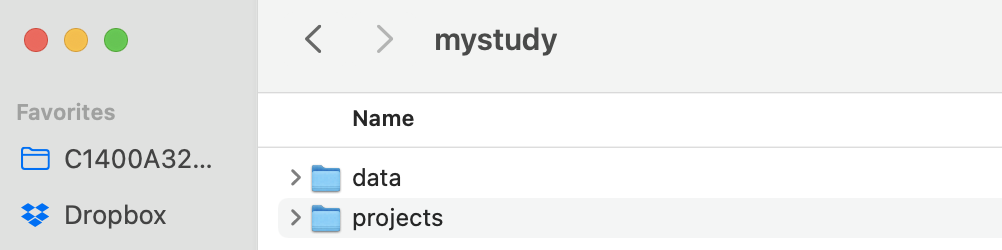
\includegraphics[width=0.75\linewidth]{images/mystudy-dir-fig1} \caption{Example directory for `mystudy`}\label{fig:dir-fig1}
\end{figure}

Start by dividing a project into major activities. In the example abpve, the project is named \texttt{mystudy}. There is a \texttt{data} subdirectory (more in a sec), and then three major activities, each corresponding to a separate analysis: \texttt{primary-analysis},\texttt{secondary-analysis-1}, and \texttt{secondary-analysis-2}. In a real project, the names could be more informative, such as ``trachoma-qpcr''. Also, a real project might also include many additional subdirectories related to administrative and logistics activities that do not relate to data science, such as irb, travel, contracts, budget, survey forms, etc.).

Dividing files into major activities helps keep things organized for really big projects. In a multi-site study, consider including a directory for each site before splitting files into major activities. Ideally, analyses will not span major activity subdirectories in a project folder, but sometimes you can't predict/avoid that from happening.

\subsection{Second level: data}\label{second-level-data}

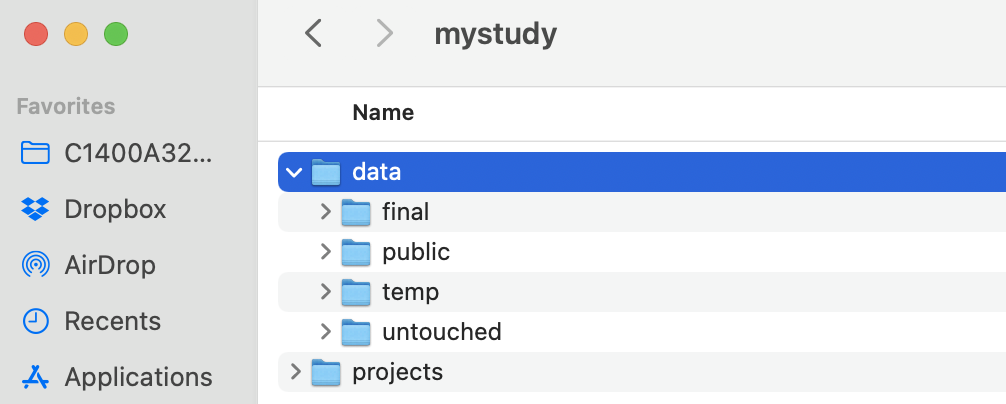
\includegraphics[width=0.75\linewidth]{images/mystudy-dir-fig2}

Each project will include a \texttt{data} directory. We recommend organizing it into 3 parts: \texttt{untouched}, \texttt{temp}, and \texttt{final}. Often, it is useful to include a fourth subdirectory called \texttt{public} for sharing public versions of datasets.

The \texttt{untouched} directory includes all untouched datasets that are used for the study. Once saved in the directory never touch them; you will read them into the work flow, but \textbf{never, ever save over them}. If the study has repeated extracts from rolling data collection or electronic health records, consider subdirectories within \texttt{untouched} that are indexed by date.

The \texttt{temp} directory (optional, not essential) includes temporary files that you might generate during the data management process. This is mainly a space for experimentation. As a rule, never save anything in the temp directory that you cannot delete. Regularly delete files in the temp directory to save disk space.

The \texttt{final} directory includes final datasets for the activity. Final datasets are de-identified and require no further processing; they are clean and ready for analysis. They should be accompanied by meta-data, which at minimum includes the data's provenance (i.e., how it was created) and what it includes (i.e., level of the data, plus variable coding/labels/descriptions). Clean/final datasets generated by one analysis might be reused in another.

\textbf{NOTE:} In very large projects, we occasionally need to further stratify the \texttt{data} directory into different subdirectories, according to data type. For example, in the AVENIR trial we had child mortality data measurements, and completely separate data from antimicrobial resistance (AMR) monitoring. These data were so myriad and different, that they needed to be curated in separate directories.

\subsection{Second level: projects}\label{second-level-projects}

We recommend maintaining a separate project subdirectory to hold each major analysis in a project. In this example, there are four workflows with generic names from the view of trial: \texttt{core-data-processing}, \texttt{primary-analysis}, \texttt{secondary-analysis-1}, \texttt{secondary-analysis-2}.

\textbf{IMPORTANT:} We recommend consolidating the core data processing for the study in its own project. \textbf{Core data processing} is data processing that creates a shared asset across multiple, downstream analyses. It includes the scripts for the data processing workflow that take data from \texttt{untouched} to \texttt{final} in the previous section.

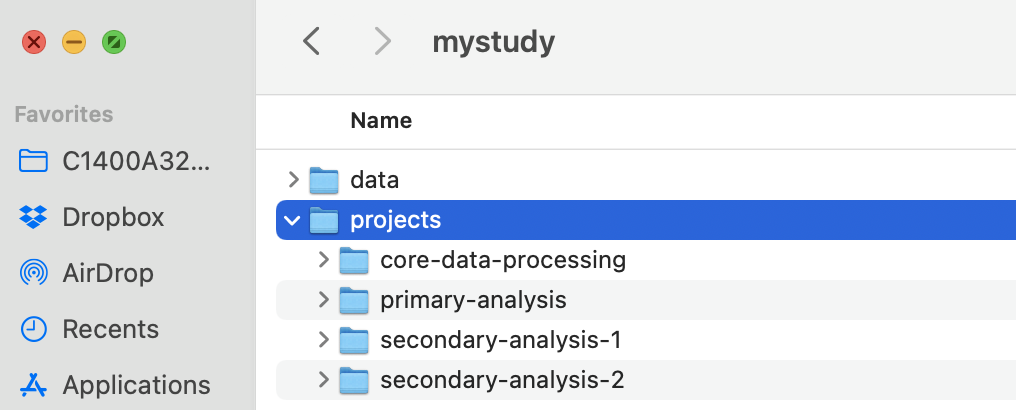
\includegraphics[width=0.75\linewidth]{images/mystudy-dir-fig3}

Think of each analysis as the scope of all of the work for a single, published paper. We recommend dividing the analysis project into a space for computational notebooks / scripts (i.e., a \texttt{code\ repository}), and a second for their output. The reason for the split is to make it easier to use version control (should you choose) for the code. Version control like \texttt{git} and \texttt{GitHub} (see the \hyperref[GitHub]{Chapter on GitHub}) works well for text files but isn't really designed for binary files such as images (.png), datasets (.rds), or PDF files (.pdf). It is certainly possible to use git with those file types, but since git makes a new copy of the file every time it is changed the git repo can get horribly bloated and takes up too much space on disk. Consolidating the output into a separate directory makes it more obvious that it isn't under version control. In this example, there are separate parts for code (\texttt{R}) and output (\texttt{output}). Output could include figures, tables, or saved analysis results stored as data files (.rds or .csv). Another conventional name for the code repository is \texttt{src} as an alternative to \texttt{R} if you use other languages.

If a project creates unique datasets or relies on new data that is unique to the project and not a shared asset for the study (e.g., publicly available data), then the project itself might include a \texttt{data} subdirectory. HOWEVER, it should not include a direct copy of shared datasets stored in the \texttt{mystudy/data} repository -- be sure to keep only one copy of each shared dataset in the project.

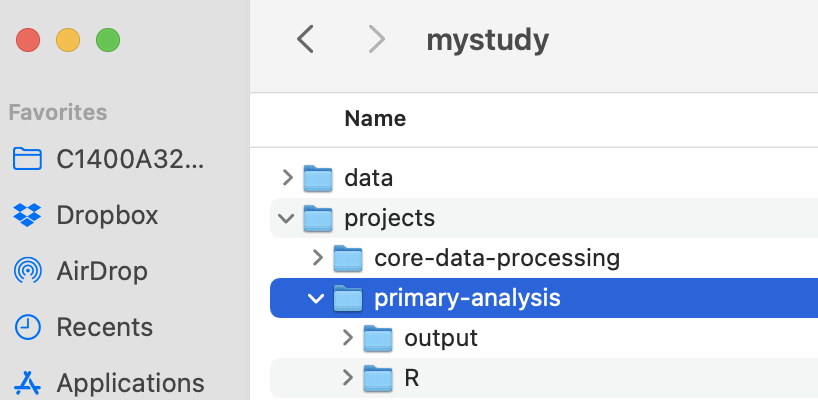
\includegraphics[width=0.75\linewidth]{images/mystudy-dir-fig4}

\begin{center}\rule{0.5\linewidth}{0.5pt}\end{center}

\textbf{Interdependence between analyses:} Sometimes a result from an analysis might be a cleaned dataset that could feed into future, distinct analyses. This is quite common, for example, in large trials where a set of baseline characteristics might be used in multiple separate papers for different endpoints, either for assessing balance of the trial population or subgroups, or used as adjustment covariates in additional analyses of the trial. In this case, the analysis-specific data processing should be \emph{moved upstream} into the \texttt{projects/core-data-processing} workflow, and should generate a shared, final dataset in the \texttt{data/final} directory.

\begin{center}\rule{0.5\linewidth}{0.5pt}\end{center}

\section{Code Repositories}\label{code-repositories}

Maintain a separate code repository for each major analysis activity (last section).

We recommend the following structure for a code repository. This is the actual repository for the \href{https://github.com/proctor-ucsf/AVENIR-primary}{AVENIR trial primary analysis}.

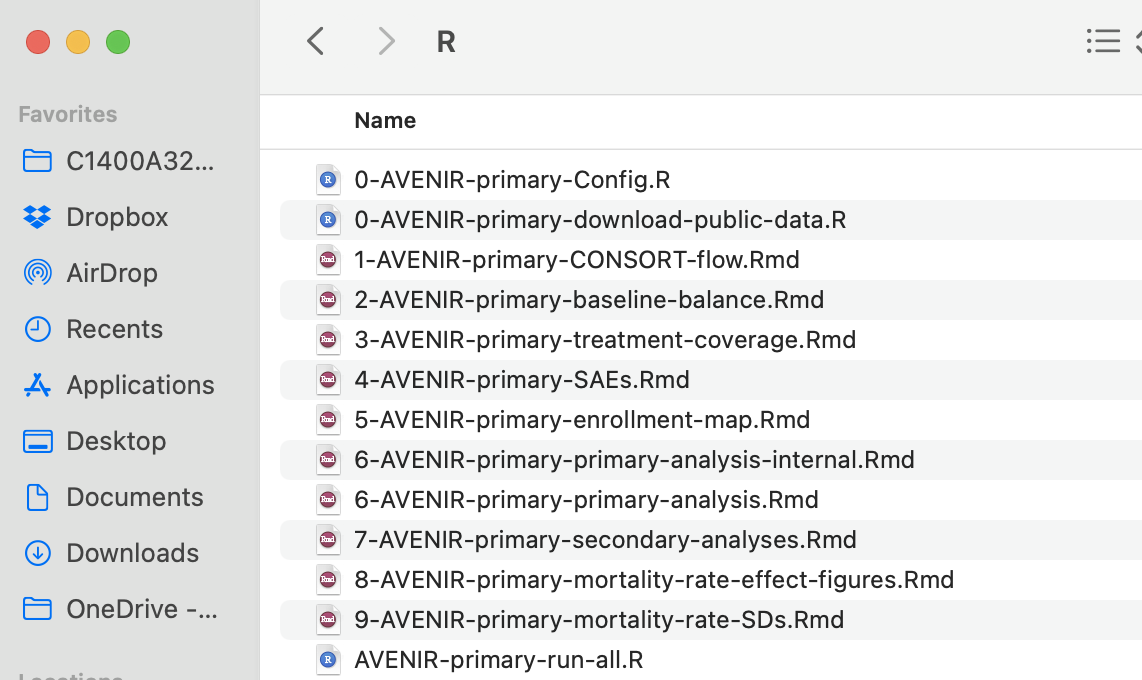
\includegraphics[width=0.75\linewidth]{images/mystudy-dir-fig5}

Note that in this example, there is no actual data processing in the project. All of the data processing was consolidated upstream in a separate \texttt{core-data-processing} project for the trial. Sometimes, an analysis/project will include limited project-specific data processing that is not shared across the trial. If project-specific data processing is required, it would be one of the first scripts in the workflow. This helps ensure work conducted in step 1 of your workflow stays upstream from all analyses (see \hyperref[workflows]{Chapter on workflows}).

In this example, there is a script that downloads public datasets into a local repository instead. Also note that in this example, all of the scripts are \texttt{.Rmd} files. R scripts \texttt{.R} are equally useful.

You can glean some important takeaways from what you \emph{do} see.

\subsection{\texorpdfstring{\texttt{.Rproj} files}{.Rproj files}}\label{rproj-files}

An ``R Project'' can be created within RStudio by going to \texttt{File\ \textgreater{}\textgreater{}\ New\ Project}. Depending on where you are with your research, choose the most appropriate option. This will save preferences, working directories, and even the results of running code/data (though we recommend starting from scratch each time you open your project, in general). Then, ensure that whenever you are working on that specific research project, you open your created project to enable the full utility of \texttt{.Rproj} files. This also automatically sets the directory to the top level of the project.

\subsection{Configuration (`config') File}\label{configuration-config-file}

This is the single most important file for your project. It will be responsible for a variety of common tasks, declare global variables, load functions, declare paths, and more. \emph{Every other file in the project} will begin with \texttt{source("0-config")}, and its role is to reduce redundancy and create an abstraction layer that allows you to make changes in one place (\texttt{0-config.R}) rather than 5 different files. To this end, paths that will be referenced in multiple scripts (e.g., a \texttt{clean\_data\_path}) can be declared in \texttt{0-config.R} and simply referred to by its variable name in scripts. If you ever want to change things, rename them, or even switch from a downsample to the full data, all you would then to need to do is modify the path in one place and the change will automatically update throughout your project. See the example config file for more details. The paths defined in the \texttt{0-config.R} file assume that users have opened the \texttt{.Rproj} file, which sets the directory to the top level of the project.

This \href{https://github.com/jadebc-berkeley/WBB-STH-Kato-Katz}{GitHub repository} that has replication files for \href{https://www.biorxiv.org/content/10.1101/629501v1}{this study} includes an example of a streamlined \texttt{config.R} file, with all packages loaded and directory references defined.

\subsection{Shared Functions File}\label{shared-functions-file}

If you write a custom function for an analysis and need to use it repeatedly across multiple analysis scripts, then it is better to consolidate it into a single shared functions script and source that file into the analysis scripts. The reason for this is that it enables you to edit the function in a single place and ensure that the changes are implemented across your entire workflow. In extreme cases, you might have so many shared functions that you need an entire subdirectory with separate scripts. \href{https://github.com/HBGD-UCB/ki-longitudinal-manuscripts/}{This repository} includes a very complex example (\texttt{0-project-functions}) of a large analysis published in a \emph{Nature} series (one of three articles: \url{https://www.nature.com/articles/s41586-023-06501-x})

\subsection{Order Files and Subdirectories}\label{order-files-and-subdirectories}

This makes the jumble of alphabetized filenames much more coherent and places similar code and files next to one another. Although sometimes there is not a linear progression from 1 to 2 to 3, in general the structure helps reflect how data flows from start to finish.

\textbf{If you take nothing else away from this guide, this is the single most helpful suggestion to make your workflow more coherent.} Often the particular order of files will be in flux until an analysis is close to completion. At that time it is important to review file order and naming and reproduce everything prior to drafting a manuscript.

\subsection{Use Bash scripts or R scripts to ensure reproducibility}\label{use-bash-scripts-or-r-scripts-to-ensure-reproducibility}

Bash scripts are useful components of a reproducible workflow. If your workflow is in R scripts, bash (\texttt{.sh}) can be useful to run the entire workflow in order. See the \hyperref[unix]{UNIX Chapter} for further details. If your workflow is mainly R markdown or a mix of \texttt{.R} and \texttt{.Rmd} files, sometimes it is easier to simply make a single R script to run the workflow. In the AVENIR example (above), that is what we used \href{https://github.com/proctor-ucsf/AVENIR-primary/blob/main/R/AVENIR-primary-run-all.R}{AVENIR-primary-run-all.R}.

\subsection{Alternative approach for code repos}\label{alternative-approach-for-code-repos}

Another approach for organizing your code repository is to name all of your scripts according to the final figure or table that they generate for a particular article. In our experience, this \emph{only} works for small projects, with a single set of coherent analyses. Here, you might have an alternative structure such as:

\begin{verbatim}
.gitignore
primary-analysis.Rproj
0-config.R
0-shared-functions.R
0-primary-analysis-run-all.sh
1-dm /
    0-dm-run-all.sh
    1-format-enrollment-data.R
    2-format-adherence-data.R
    3-format-LAZ-measurements.R
Fig1-consort.Rmd
Fig2-adherence.Rmd
Fig3-1-laz-analysis.Rmd
Fig3-2-laz-make-figure.Rmd
\end{verbatim}

There is still a need for a separate data management directory (e.g., \texttt{dm}) to ensure that workflow is upstream from the analysis (more below in \hyperref[unix]{chapter on UNIX}), but then scripts are all together with clear labels. If a figure requires two stages to the analysis, then you can name them sequentially, such as \texttt{Fig3-1-laz-analysis.Rmd}, \texttt{Fig3-2-laz-make-figure.Rmd}. There is no way to divine how all of the analyses will neatly fit into files that correspond to separate figures. Instead, they will converge on these file names through the writing process, often through comsolidation or recombination.

One example of a small repo is here:
\url{https://github.com/ben-arnold/enterics-seroepi}

\chapter{Coding Practices}\label{codingpractices}

\emph{Contributors: Kunal Mishra, Jade Benjamin-Chung, Ben Arnold}

\section{Organizing scripts}\label{organizing-scripts}

Just as your data ``flows'' through your project, data should flow naturally through a script. Very generally, you want to:

\begin{enumerate}
\def\labelenumi{\arabic{enumi}.}
\tightlist
\item
  describe the work completed in the script in a comment header
\item
  source your configuration file (\texttt{0-config.R})
\item
  load all of your data
\item
  do all your analysis/computation in order
\item
  save your results
\end{enumerate}

Each section should be ``chunked together'' using comments, often with many chunks in a single section. See \href{https://github.com/kmishra9/Flu-Absenteeism/blob/master/Master's%20Thesis%20-%20Spatial%20Epidemiology%20of%20Influenza/2a%20-%20Statistical-Inputs.R}{this file} for a good example of how to cleanly organize a file in a way that follows this ``flow'' and functionally separate pieces of code that are doing different things. \href{https://github.com/ben-arnold/enterics-seroepi/blob/master/R/Fig1-haiti-ab-distributions.Rmd}{This is another example} in a \texttt{.Rmd} format, where chunking is made even more obvious by the interleaving of markdown text and R code in the same notebook file.

\section{Documenting your code}\label{documenting-your-code}

\subsection{File headers}\label{file-headers}

Every file in a project should have a header that allows it to be interpreted on its own. It should include the name of the project and a short description for what this file (among the many in your project) does specifically. You may optionally wish to include the inputs and outputs of the script as well, though the next section makes this significantly less necessary. It can be very helpful to include your name and email address as well so others can identify who wrote the code. This is unnecessary if you are using version control (\texttt{git/GitHub}) becuase that information will be tracked by commits.

\begin{verbatim}
#-------------------------------------------------------------------------------
# @Organization - Example Organization
# @Project - Example Project
# @Author - Your name, and possibly email address (if appropriate)
# @Description - This file is responsible for [...]
#-------------------------------------------------------------------------------
\end{verbatim}

Consider using RStudio's \href{https://support.rstudio.com/hc/en-us/articles/200484568-Code-Folding-and-Sections}{code folding} feature to collapse and expand different sections of your code. Any comment line with at least four trailing dashes (-), equal signs (=), or pound signs (\#) automatically creates a code section. Delimiters for chunks are a personal preference and all work equally well. For example:

\begin{verbatim}
# Section 1 ------------------
\end{verbatim}

works equally well as

\begin{verbatim}
##############################
# Section 1 ##################
##############################
\end{verbatim}

\subsection{Comments in the body of your script}\label{comments-in-the-body-of-your-script}

Commenting your code is an important part of reproducibility and helps document your code for the future. When things change or break, you'll be thankful for comments. When you revisit code you wrote two years earlier, you'll be thankful for comments. There's no need to comment excessively or unnecessarily, but a comment describing what a large or complex chunk of code does is always helpful. See \href{https://github.com/kmishra9/Flu-Absenteeism/blob/master/Master's%20Thesis%20-%20Spatial%20Epidemiology%20of%20Influenza/1b%20-%20Map-Management.R}{this file} for an example of how to comment your code and notice that comments are always in the form of:

\texttt{\#\ This\ is\ a\ comment\ -\/-\ first\ letter\ is\ capitalized\ and\ spaced\ away\ from\ the\ pound\ sign}

\subsection{Function documentation}\label{function-documentation}

Every function you write must include a header to document its purpose, inputs, and outputs. For any reproducible workflows, they are essential, because R is dynamically typed. This means, you can pass a \texttt{string} into an argument that is meant to be a \texttt{data.table}, or a \texttt{list} into an argument meant for a \texttt{tibble}. It is the responsibility of a function's author to document what each argument is meant to do and its basic type. This is an example for documenting a function (inspired by \href{https://www.oracle.com/technetwork/java/javase/documentation/index-137868.html#format}{JavaDocs}, R's \href{https://blog.rstudio.com/2018/10/23/rstudio-1-2-preview-plumber-integration/}{Plumber API docs}, and \href{https://kbroman.org/pkg_primer/pages/docs.html}{Roxygen2}):

\begin{verbatim}
#-----------------------------------------------------------------------------
# Documentation: calc_fluseas_mean
# Usage: calc_fluseas_mean(data, yname)
# @description: Make a dataframe with rows for flu season and site
#               and the number of patients with an outcome, the total patients,
#               and the percent of patients with the outcome

# Arguments/Options:
# @param data: a data frame with variables flu_season, site, studyID, and yname
# @param yname: a string for the outcome name
# @param silent: a boolean specifying whether the function shouldn't output anything to the console (DEFAULT: TRUE)

# @return: the dataframe as described above
# @output: prints the data frame described above if silent is not True
#-----------------------------------------------------------------------------

calc_fluseas_mean = function(data, yname, silent = TRUE) {
 ### function code here 

}
\end{verbatim}

The header tells you what the function does, its various inputs, and how you might go about using the function to do what you want. Also notice that all optional arguments (i.e.~ones with pre-specified defaults) follow arguments that require user input.

\begin{itemize}
\item
  \textbf{Note}: As someone trying to call a function, it is possible to access a function's documentation (and internal code) by \texttt{CMD-Left-Click}ing the function's name in RStudio
\item
  \textbf{Note}: Depending on how important your function is, the complexity of your function code, and the complexity of different types of data in your project, you can also add ``type-checking'' to your function with the \texttt{assertthat::assert\_that()} function. You can, for example, \texttt{assert\_that(is.data.frame(statistical\_input))}, which will ensure that collaborators or reviewers of your project attempting to use your function are using it in the way that it is intended by calling it with (at the minimum) the correct type of arguments. You can extend this to ensure that certain assumptions regarding the inputs are fulfilled as well (i.e.~that \texttt{time\_column}, \texttt{location\_column}, \texttt{value\_column}, and \texttt{population\_column} all exist within the \texttt{statistical\_input} tibble).
\end{itemize}

\section{Object naming}\label{object-naming}

Generally we recommend using nouns for objects and verbs for functions. This is because functions are performing actions, while objects are not.

Try to make your variable names both more expressive and more explicit. Being a bit more verbose is useful and easy in the age of autocompletion! For example, instead of naming a variable \texttt{vaxcov\_1718}, try naming it \texttt{vaccination\_coverage\_2017\_18}. Similarly, \texttt{flu\_res} could be named \texttt{absentee\_flu\_residuals}, making your code more readable and explicit.

\begin{itemize}
\tightlist
\item
  For more help, check out \href{https://spin.atomicobject.com/2017/11/01/good-variable-names/}{Be Expressive: How to Give Your Variables Better Names}
\end{itemize}

We recommend you use \textbf{Snake\_Case}.

\begin{itemize}
\item
  Base R allows \texttt{.} in variable names and functions (such as \texttt{read.csv()}), but this goes against best practices for variable naming in many other coding languages. For consistency's sake, \texttt{snake\_case} has been adopted across languages, and modern packages and functions typically use it (i.e.~\texttt{readr::read\_csv()}). As a very general rule of thumb, if a package you're using doesn't use \texttt{snake\_case}, there may be an updated version or more modern package that \emph{does}, bringing with it the variety of performance improvements and bug fixes inherent in more mature and modern software.
\item
  \textbf{Note}: you may also see \texttt{camelCase} throughout the R code you come across. This is \emph{okay} but not ideal -- try to stay consistent across all your code with \texttt{snake\_case}.
\item
  \textbf{Note}: there is nothing inherently wrong with using \texttt{.} in variable names, just that it goes against style best practices that are cropping up in data science, so its worth getting rid of these bad habits now.
\end{itemize}

\section{Function calls}\label{function-calls}

In a function call, use ``named arguments'' and separate arguments by to make your code more readable.

Here's an example of what not to do when calling the function a function \texttt{calc\_fluseas\_mean} (defined above):

\begin{verbatim}
mean_Y = calc_fluseas_mean(flu_data, "maari_yn", FALSE)
\end{verbatim}

And here it is again using the best practices we've outlined:

\begin{verbatim}
mean_Y = calc_fluseas_mean(
  data = flu_data, 
  yname = "maari_yn",
  silent = FALSE
)
\end{verbatim}

\section{\texorpdfstring{The \texttt{here} package}{The here package}}\label{the-here-package}

The \texttt{here} package is one great R package that helps multiple collaborators deal with the mess that is working directories within an R project structure. Let's say we have an R project at the path \texttt{/home/oski/Some-R-Project}. My collaborator might clone the repository and work with it at some other path, such as \texttt{/home/bear/R-Code/Some-R-Project}. Dealing with working directories and paths explicitly can be a very large pain, and as you might imagine, setting up a Config with paths requires those paths to flexibly work for all contributors to a project. This is where the \texttt{here} package comes in and this a \href{https://github.com/jennybc/here_here}{great vignette describing it}.

For more motivation on why you should use the \texttt{here} and R projects (\texttt{.Rproj}), read this excellent blog post from \href{https://www.tidyverse.org/articles/2017/12/workflow-vs-script/}{Tidyverse}.

\section{Tidyverse}\label{tidyverse}

Throughout this document there have been references to the Tidyverse, but this section is to explicitly show you how to transform your Base R tendencies to Tidyverse (or Data.Table, Tidyverse's performance-optimized competitor). For most of our work that does not utilize very large datasets, we recommend that you code in Tidyverse rather than Base R. Tidyverse is quickly becoming \href{https://rviews.rstudio.com/2017/06/08/what-is-the-tidyverse/}{the gold standard} in R data analysis and modern data science packages and code should use Tidyverse style and packages unless there's a significant reason not to (i.e.~big data pipelines that would benefit from Data.Table's performance optimizations).

The package author has published a \href{https://r4ds.had.co.nz/}{great textbook on R for Data Science}, which leans heavily on many Tidyverse packages and may be worth checking out.

The following list is not exhaustive, but is a compact overview to begin to translate Base R into something better:

\begin{longtable}[]{@{}
  >{\raggedright\arraybackslash}p{(\columnwidth - 2\tabcolsep) * \real{0.5000}}
  >{\raggedright\arraybackslash}p{(\columnwidth - 2\tabcolsep) * \real{0.5000}}@{}}
\toprule\noalign{}
\begin{minipage}[b]{\linewidth}\raggedright
Base R
\end{minipage} & \begin{minipage}[b]{\linewidth}\raggedright
Better Style, Performance, and Utility
\end{minipage} \\
\midrule\noalign{}
\endhead
\bottomrule\noalign{}
\endlastfoot
\_ & \_ \\
\texttt{read.csv()} & \texttt{readr::read\_csv()} or \texttt{data.table::fread()} \\
\texttt{write.csv()} & \texttt{readr::write\_csv()} or \texttt{data.table::fwrite()} \\
\texttt{readRDS} & \texttt{readr::read\_rds()} \\
\texttt{saveRDS()} & \texttt{readr::write\_rds()} \\
\_ & \_ \\
\texttt{data.frame()} & \texttt{tibble::tibble()} or \texttt{data.table::data.table()} \\
\texttt{rbind()} & \texttt{dplyr::bind\_rows()} \\
\texttt{cbind()} & \texttt{dplyr::bind\_cols()} \\
\texttt{df\$some\_column} & \texttt{df\ \%\textgreater{}\%\ dplyr::pull(some\_column)} \\
\texttt{df\$some\_column\ =\ ...} & \texttt{df\ \%\textgreater{}\%\ dplyr::mutate(some\_column\ =\ ...)} \\
\texttt{df{[}get\_rows\_condition,{]}} & \texttt{df\ \%\textgreater{}\%\ dplyr::filter(get\_rows\_condition)} \\
\texttt{df{[},c(col1,\ col2){]}} & \texttt{df\ \%\textgreater{}\%\ dplyr::select(col1,\ col2)} \\
\texttt{merge(df1,\ df2,\ by\ =\ ...,\ all.x\ =\ ...,\ all.y\ =\ ...)} & \texttt{df1\ \%\textgreater{}\%\ dplyr::left\_join(df2,\ by\ =\ ...)} or \texttt{dplyr::full\_join} or \texttt{dplyr::inner\_join} or \texttt{dplyr::right\_join} \\
\_ & \_ \\
\texttt{str()} & \texttt{dplyr::glimpse()} \\
\texttt{grep(pattern,\ x)} & \texttt{stringr::str\_which(string,\ pattern)} \\
\texttt{gsub(pattern,\ replacement,\ x)} & \texttt{stringr::str\_replace(string,\ pattern,\ replacement)} \\
\texttt{ifelse(test\_expression,\ yes,\ no)} & \texttt{if\_else(condition,\ true,\ false)} \\
Nested: \texttt{ifelse(test\_expression1,\ yes1,\ ifelse(test\_expression2,\ yes2,\ ifelse(test\_expression3,\ yes3,\ no)))} & \texttt{case\_when(test\_expression1\ \textasciitilde{}\ yes1,\ \ test\_expression2\ \textasciitilde{}\ yes2,\ test\_expression3\ \textasciitilde{}\ yes3,\ TRUE\ \textasciitilde{}\ no)} \\
\texttt{proc.time()} & \texttt{tictoc::tic()} and \texttt{tictoc::toc()} \\
\texttt{stopifnot()} & \texttt{assertthat::assert\_that()} or \texttt{assertthat::see\_if()} or \texttt{assertthat::validate\_that()} \\
\end{longtable}

For a more extensive set of syntactical translations to Tidyverse, you can check out \href{https://tavareshugo.github.io/data_carpentry_extras/base-r_tidyverse_equivalents/base-r_tidyverse_equivalents.html#reshaping_data}{this document}.

Working with Tidyverse within functions can be somewhat of a pain due to non-standard evaluation (NSE) semantics. If you're an avid function writer, we'd recommend checking out the following resources:

\begin{itemize}
\tightlist
\item
  \href{https://www.youtube.com/watch?v=nERXS3ssntw}{Tidy Eval in 5 Minutes} (video)
\item
  \href{https://tidyeval.tidyverse.org/index.html}{Tidy Evaluation} (e-book)
\item
  \href{https://www.brodrigues.co/blog/2016-07-18-data-frame-columns-as-arguments-to-dplyr-functions/}{Data Frame Columns as Arguments to Dplyr Functions} (blog)
\item
  \href{https://stackoverflow.com/questions/28125816/r-standard-evaluation-for-join-dplyr}{Standard Evaluation for *\_join} (stackoverflow)
\item
  \href{https://dplyr.tidyverse.org/articles/programming.html}{Programming with dplyr} (package vignette)
\end{itemize}

\section{Coding with R and Python}\label{coding-with-r-and-python}

If you're using both R and Python, you may wish to check out the \href{https://www.rdocumentation.org/packages/feather/versions/0.3.3}{Feather package} for exchanging data between the two languages \href{https://blog.rstudio.com/2016/03/29/feather/}{extremely quickly}.

\chapter{Coding Style}\label{codingstyle}

\emph{Contributors: Kunal Mishra, Jade Benjamin-Chung, and Ben Arnold}

\section{Line breaks}\label{line-breaks}

\begin{itemize}
\item
  For \texttt{ggplot} calls and \texttt{dplyr} pipelines, do not crowd single lines. Here are some nontrivial examples of ``beautiful'' pipelines, where beauty is defined by coherence:

\begin{verbatim}
# Example 1
school_names <- list(
  OUSD_school_names = absentee_all %>%
    filter(dist.n == 1) %>%
    pull(school) %>%
    unique() %>%
    sort(),

  WCCSD_school_names <- absentee_all %>%
    filter(dist.n == 0) %>%
    pull(school) %>%
    unique() %>%
    sort()
)
\end{verbatim}

\begin{verbatim}
# Example 2
absentee_all <- fread(file = raw_data_path) %>%
  mutate(program = case_when(schoolyr %in% pre_program_schoolyrs ~ 0,
                             schoolyr %in% program_schoolyrs ~ 1)) %>%
  mutate(period = case_when(schoolyr %in% pre_program_schoolyrs ~ 0,
                            schoolyr %in% LAIV_schoolyrs ~ 1,
                            schoolyr %in% IIV_schoolyrs ~ 2)) %>%
  filter(schoolyr != "2017-18")
\end{verbatim}

  And of a complex \texttt{ggplot} call:

\begin{verbatim}
# Example 3
ggplot(data=data,
       mapping=aes_string(x="year", y="rd", group=group)) +

  geom_point(mapping=aes_string(col=group, shape=group),
             position=position_dodge(width=0.2),
             size=2.5) +

  geom_errorbar(mapping=aes_string(ymin="lb", ymax="ub", col=group),
                position=position_dodge(width=0.2),
                width=0.2) +

  geom_point(position=position_dodge(width=0.2),
             size=2.5) +

  geom_errorbar(mapping=aes(ymin=lb, ymax=ub),
                position=position_dodge(width=0.2),
                width=0.1) +

  scale_y_continuous(limits=limits,
                     breaks=breaks,
                     labels=breaks) +

  scale_color_manual(std_legend_title,values=cols,labels=legend_label) +
  scale_shape_manual(std_legend_title,values=shapes, labels=legend_label) +
  geom_hline(yintercept=0, linetype="dashed") +
  xlab("Program year") +
  ylab(yaxis_lab) +
  theme_complete_bw() +
  theme(strip.text.x = element_text(size = 14),
        axis.text.x = element_text(size = 12)) +
  ggtitle(title)
\end{verbatim}
\end{itemize}

Imagine (or perhaps mournfully recall) the mess that can occur when you don't strictly style a complicated \texttt{ggplot} call. Trying to fix bugs and ensure your code is working can be a nightmare. Now imagine trying to do it with the same code 6 months after you've written it. Invest the time now and reap the rewards as the code practically explains itself, line by line.

\section{Automated Tools for Style and Project Workflow}\label{automated-tools-for-style-and-project-workflow}

\subsection{Styling}\label{styling}

\begin{enumerate}
\def\labelenumi{\arabic{enumi}.}
\item
  \textbf{Code Autoformatting} - RStudio includes a fantastic built-in utility (keyboard shortcut: \texttt{CMD-Shift-A}) for autoformatting highlighted chunks of code to fit many of the best practices listed here. It generally makes code more readable and fixes a lot of the small things you may not feel like fixing yourself. Try it out as a ``first pass'' on some code of yours that \emph{doesn't} follow many of these best practices!
\item
  \textbf{Assignment Aligner} - A \href{https://www.r-bloggers.com/align-assign-rstudio-addin-to-align-assignment-operators/}{cool R package} allows you to very powerfully format large chunks of assignment code to be much cleaner and much more readable. Follow the linked instructions and create a keyboard shortcut of your choosing (recommendation: \texttt{CMD-Shift-Z}). Here is an example of how assignment aligning can dramatically improve code readability:
\end{enumerate}

\begin{verbatim}
# Before
OUSD_not_found_aliases <- list(
  "Brookfield Village Elementary" = str_subset(string = OUSD_school_shapes$schnam, pattern = "Brookfield"),
  "Carl Munck Elementary" = str_subset(string = OUSD_school_shapes$schnam, pattern = "Munck"),
  "Community United Elementary School" = str_subset(string = OUSD_school_shapes$schnam, pattern = "Community United"),
  "East Oakland PRIDE Elementary" = str_subset(string = OUSD_school_shapes$schnam, pattern = "East Oakland Pride"),
  "EnCompass Academy" = str_subset(string = OUSD_school_shapes$schnam, pattern = "EnCompass"),
  "Global Family School" = str_subset(string = OUSD_school_shapes$schnam, pattern = "Global"),
  "International Community School" = str_subset(string = OUSD_school_shapes$schnam, pattern = "International Community"),
  "Madison Park Lower Campus" = "Madison Park Academy TK-5",
  "Manzanita Community School" = str_subset(string = OUSD_school_shapes$schnam, pattern = "Manzanita Community"),
  "Martin Luther King Jr Elementary" = str_subset(string = OUSD_school_shapes$schnam, pattern = "King"),
  "PLACE @ Prescott" = "Preparatory Literary Academy of Cultural Excellence",
  "RISE Community School" = str_subset(string = OUSD_school_shapes$schnam, pattern = "Rise Community")
)
\end{verbatim}

\begin{verbatim}
# After
OUSD_not_found_aliases <- list(
  "Brookfield Village Elementary"      = str_subset(string = OUSD_school_shapes$schnam, pattern = "Brookfield"),
  "Carl Munck Elementary"              = str_subset(string = OUSD_school_shapes$schnam, pattern = "Munck"),
  "Community United Elementary School" = str_subset(string = OUSD_school_shapes$schnam, pattern = "Community United"),
  "East Oakland PRIDE Elementary"      = str_subset(string = OUSD_school_shapes$schnam, pattern = "East Oakland Pride"),
  "EnCompass Academy"                  = str_subset(string = OUSD_school_shapes$schnam, pattern = "EnCompass"),
  "Global Family School"               = str_subset(string = OUSD_school_shapes$schnam, pattern = "Global"),
  "International Community School"     = str_subset(string = OUSD_school_shapes$schnam, pattern = "International Community"),
  "Madison Park Lower Campus"          = "Madison Park Academy TK-5",
  "Manzanita Community School"         = str_subset(string = OUSD_school_shapes$schnam, pattern = "Manzanita Community"),
  "Martin Luther King Jr Elementary"   = str_subset(string = OUSD_school_shapes$schnam, pattern = "King"),
  "PLACE @ Prescott"                   = "Preparatory Literary Academy of Cultural Excellence",
  "RISE Community School"              = str_subset(string = OUSD_school_shapes$schnam, pattern = "Rise Community")
)
\end{verbatim}

\begin{enumerate}
\def\labelenumi{\arabic{enumi}.}
\setcounter{enumi}{2}
\tightlist
\item
  \textbf{StyleR} - Another \href{https://www.tidyverse.org/articles/2017/12/styler-1.0.0/}{cool R package from the Tidyverse} that can be powerful and used as a first pass on entire projects that need refactoring. The most useful function of the package is the \texttt{style\_dir} function, which will style all files within a given directory. See the \href{https://www.rdocumentation.org/packages/styler/versions/1.1.0/topics/style_dir}{function's documentation} and the vignette linked above for more details.

  \begin{itemize}
  \tightlist
  \item
    \textbf{Note}: The default Tidyverse styler is subtly different from some of the things we've advocated for in this document. Most notably we differ with regards to the number of spaces before/after ``tokens'' (i.e.~Assignment Aligner add spaces before \texttt{=} signs to align them properly). For this reason, we'd recommend the following: \texttt{style\_dir(path\ =\ ...,\ scope\ =\ "line\_breaks",\ strict\ =\ FALSE)}. You can also customize StyleR \href{http://styler.r-lib.org/articles/customizing_styler.html}{even more} if you're really hardcore.
  \item
    \textbf{Note}: As is mentioned in the package vignette linked above, StyleR modifies things \emph{in-place}, meaning it overwrites your existing code and replaces it with the updated, properly styled code. This makes it a good fit on projects \emph{with version control}, but if you don't have backups or a good way to revert back to the intial code, I wouldn't recommend going this route.
  \end{itemize}
\end{enumerate}

\chapter{Data Wrangling}\label{datawrangling}

\emph{Contributors: Kunal Mishra, Jade Benjamin-Chung, Ben Arnold}

\section{Overview}\label{overview}

Processing data from raw inputs to final data for analysis is the foundation of the data science \hyperref[workflows]{workflow}. ``Management'' is a bad word in both academia and hip parts of the private sector, so what used to be called ``data management'' is now called ``data wrangling'' or ``data munging''.

By any name, it is by far the most tedious and time consuming step in the data analysis workflow. Data wrangling is also the most error prone. Errors are likely because data processing usually requires hundreds or thousands of lines of code. Generating final datasets often requires programmers to merge and append multiple different raw datasets; often, the process requires them to re-shape the data from wide format to long format.

Read the chapters on \href{https://r4ds.had.co.nz/}{Data Wrangling} in \emph{R for Data Science}. That book covers the foundational skills and know-how.

Here, we provide some additional recommendations for best practices related to data wrangling and highlight a few topics not covered in the excellent R for Data Science book.

\section{Cardinal rule}\label{cardinal-rule}

\begin{center}\rule{0.5\linewidth}{0.5pt}\end{center}

\begin{quote}
\emph{\textbf{Cardinal rule of data wrangling:} NEVER alter untouched datasets}
\end{quote}

\begin{center}\rule{0.5\linewidth}{0.5pt}\end{center}

Untouched datasets include data output from data collection software, distributed by the data team, outside collaborators, or downloaded from a data repository. They should be left untouched. All data cleaning and processing activities should read in untouched data and output either temporary files or final datasets. Never, ever overwrite an untouched dataset.

\section{Data input/output (I/O)}\label{data-inputoutput-io}

Read the \href{https://r4ds.had.co.nz/data-import.html}{Data Import} section of \emph{R for Data Science}.

\subsection{Excel files}\label{excel-files}

Often collaborators share data as Excel files (\texttt{.xlsx}). In this case, we recommend making a copy of the file in the untouched repository and converting it into a \texttt{.csv} file (one per tab) to input into the data processing workflow.

This step should mark the end of your use of Excel in your data analysis, aside from inspecting \texttt{.csv} files. Excel is extremely error prone because it does not have good fidelity with variable types (e.g., dates, leading zeros), and has no real programmatic interface (VBA?). Avoid it. We can find no compelling case for its use in data science.

\subsection{\texorpdfstring{\texttt{.RDS} vs \texttt{.RData} Files}{.RDS vs .RData Files}}\label{rds-vs-.rdata-files}

One of the most common ways to load and save data in Base R is with the \texttt{load()} and \texttt{save()} functions to serialize multiple objects in a single \texttt{.RData} file. The biggest problems with this practice include an inability to control the names of things getting loaded in, the inherent confusion this creates in understanding older code, and the inability to load individual elements of a saved file. For this, we recommend using the RDS format to save R objects using \texttt{saveRDS()} and its complement \texttt{readRDS()}.

\begin{itemize}
\item
  \textbf{Note}: if you have many related R objects you would have otherwise saved all together using the \texttt{save} function, the functional equivalent with \texttt{RDS} would be to create a (named) list containing each of these objects, and saving it.
\item
  \textbf{Note}: there is an important caveat for \texttt{.rds} files: they are not automatically backward compatible across different versions of R! So, while they are very useful in general, beware. See, for example, this thread on \href{https://stackoverflow.com/questions/56704638/write-a-file-using-saverds-so-that-it-is-backwards-compatible-with-old-versi}{StackExchange}. \texttt{.csv} files embed slightly less information (typically), but are more stable across different versions of R.
\end{itemize}

\subsection{\texorpdfstring{\texttt{.CSV} Files}{.CSV Files}}\label{csv-files}

Once again, the \texttt{readr} package as part of the Tidvyerse is great, with a much faster \texttt{read\_csv()} than Base R's \texttt{read.csv()}. For massive CSVs (\textgreater{} 5 GB), you'll find \texttt{data.table::fread()} to be the fastest CSV reader in any data science language out there. For writing CSVs, \texttt{readr::write\_csv()} and \texttt{data.table::fwrite()} outclass Base R's \texttt{write.csv()} by a significant margin as well.

\section{Documenting datasets}\label{documenting-datasets}

Datasets need to have metadata (documentation) associated with them to help people understand them. Well documented datasets save an enormous amount of time because it helps avoid lots of back-and-forth with new people orienting themselves with the data. This applies to both private and public data used in your work flow.

Each raw and final dataset should include a codebook. Sometimes survey instruments or electronic data capture schematics can stand-in for raw dataset codebooks, as long as that information is stored alongside the raw data!

The file \href{https://github.com/ben-arnold/enterics-seroepi/blob/master/data/asembo_analysis_codebook.txt}{asembo\_analysis\_codebook.txt} provides one example of what a codebook for a simple, final dataset could contain.

For complex studies with multiple, relational data files, it is exceptionally helpful to also include a README overview in plain text or markdown that explains the relationships between the datasets. Here is an example from the WASH Benefits Bangladesh trial primary outcomes analysis: \href{https://osf.io/v3nfs/}{README-WBB-primary-outcomes-datasets.md}.

\section{Mapping data from untouched -\textgreater{} final}\label{mapping-data-from-untouched---final}

An important step for the data processing is to come up with a plan for which final datasets you want to create.

Best pracice is to scope out the flow of data from the original forms/modules/tables at the time of data capture to the final datasets planned for the analysis, and ensure that there is a \texttt{Key} linking each table needed to create the final analysis datasets.

These are probably the two most common models for the end product:

\begin{longtable}[]{@{}
  >{\raggedright\arraybackslash}p{(\columnwidth - 2\tabcolsep) * \real{0.1923}}
  >{\raggedright\arraybackslash}p{(\columnwidth - 2\tabcolsep) * \real{0.8077}}@{}}
\toprule\noalign{}
\endhead
\bottomrule\noalign{}
\endlastfoot
Single Massive Dataset & A single, large, final dataset for the whole project with potentially multiple levels of data (e.g., household, individual) and hundreds or thousands of variables. \\
Multiple Relational datasets & Multiple relational datasets, each tailored to a specific type of data collected in the study. Smaller, relational datasets can be recombined as needed for analyses. \\
\end{longtable}

We strongly recommend using the second model, relational data tables, in almost every case. The chapter on \href{https://r4ds.had.co.nz/relational-data.html}{Relational Data} in R for Data Science explains details.

\begin{quote}
Rationale: If you create a single massive dataset that includes information at multiple levels, then it can create challenges. First, the datasets are unwieldy, often consisting of hundreds or thousands of variables; this makes it difficult to find variables, difficult to view the data through a software browser, and easy to forget about variables. \emph{But there are bigger problems}. Datasets with an exceptionally large number of variables or multiple levels of data in the same file make it difficult to visually detect pathological problems in the data (e.g., unexpected missing values). For studies that include data from multiple levels (e.g., communities, households, individuals) the inclusion of multiple types of data in the same file makes analyses error prone because it requires the programmer to keep track of when variables include duplicated observations. For example, the inclusion of household characteristics in an individual-level data file means that if there are multiple individuals per household, that simple means of household characteristics cannot be calculated without first restricting the file to unique observations at the household level.
\end{quote}

\section{Relational data}\label{relational-data}

Refer to \href{https://r4ds.had.co.nz/relational-data.html}{Relational Data} in \emph{R for Data Science} for a good example of what a good relational database can look like.

\textbf{Important}: For a set of relational tables to work, you must ensure that each table relates to another with a unique \texttt{Key}. For example, a child-level dataset must also include IDs for household- or cluster to be merged to household or cluster level data.

Practical advice on \texttt{Key} variables / IDs used to link datasets. Numeric IDs can occasionally cause problems with merges due to machine rounding errors so character values can sometimes be a good alternative. Whatever format you use, ensure that they do not in some way encode identifying information (e.g., using a social security number or medical record number would be a poor choice of ID for a final dataset).

\section{Be careful with joins / merges}\label{be-careful-with-joins-merges}

Experience shows that merging datasets is one of the most error prone steps in data wrangling. Merges can be particularly tricky for less experienced programmers. Errors are likely early in the data processing work flow, and less likely when merging final datasets with clean key variables (IDs) and clear relationships between datasets. Carefully check each merge to ensure it is working as you expect.

\begin{quote}
\textbf{ESSENTIAL READING:} \href{https://r4ds.had.co.nz/relational-data.html#join-problems}{Join Problems} in \emph{R for Data Science}
\end{quote}

In the Stata software there is a really nice feature with \texttt{merge} that allows you to specify the type of merge/join and then examine the diagnostics of that merge.

Although R does not have a similarly nice feature at this time, the different \texttt{join} functions in the \texttt{dplyr} package provide all of the tools you need to correctly join your data.

In our experience, the two most common types of joins in our work are mutating joins and filtering joints. (from the \emph{R for Data Science} book):

\begin{quote}
\textbf{Mutating joins}: add new variables to one data frame from matching observations in another.
\end{quote}

\begin{quote}
\textbf{Filtering joins}: filter observations from one data frame based on whether or not they match an observation in the other table.
\end{quote}

Familiarize yourself with these types of operations. The \href{https://r4ds.had.co.nz/relational-data.html}{Relational data} chapter of \emph{R for Data Science} includes details.

\section{Reshaping data}\label{reshaping-data}

The \texttt{dplyr} package introduced the \texttt{pivot\_wider} and \texttt{pivot\_longer} functions in 2019. They make reshaping data dramatically easier than any previous functions, including \texttt{reshape()} (base R) or \texttt{gather}/\texttt{spread} (Tidyverse). This excellent article includes details:

\url{https://tidyr.tidyverse.org/dev/articles/pivot.html}

\section{Data cleaning}\label{data-cleaning}

Data cleaning is typically an iterative process that you should conduct on a variable-by-variable basis. Occasionally it is useful to clean an entire questionnaire module at the same time since variables in the same module can be related to one another, and since it can help to proceed through the cleaning process in well-defined chunks. I find it helpful to have a copy of the survey questionnaire (if relevant) handy while cleaning specific variables. This enables you to check skip patterns and codes in the survey against the dataset.

We don't have a lot of general advice for data cleaning except the following. First, there is something to be said for ``trolling'' (in the fishing sense) or visually scrolling through parts of the dataset to see what the data look like and to make sure you have a feel for how information is stored in different variables (e.g., are missing values coded or simply recored as ``\texttt{.}'' or \texttt{NA}). Use the \texttt{View()} utility in \texttt{RStudio} to look at your data often during the cleaning process. Second, it can be helpful to consolidate all data cleaning into a single program for each dataset. The data cleaning program corrects entry errors, labels variables, formats variables, and outputs either a temporary or final dataset (but does not, ever, overwrite the untouched data). As noted in the \hyperref[workflows]{Workflows} chapter, \emph{key data processing should be done once, at the earliest possible place in the workflow}.

\chapter{Making Data Public}\label{publicdata}

\emph{Contributors: Fanice Nyatigo, Ben Arnold}

\section{Overview}\label{overview-1}

\begin{center}\rule{0.5\linewidth}{0.5pt}\end{center}

\begin{quote}
\emph{\textbf{Warning! } \textbf{NEVER} push a dataset into the public domain (e.g., GitHub, OSF) without first checking with Ben to ensure that it is appropriately de-identified and we have approval from the sponsor and/or human subjects review board to do so. For example, we will need to re-code participant IDs (even if they contain no identifying information) before making data public to completely break the link between IDs and identifiable information stored on our servers. }
\end{quote}

\begin{center}\rule{0.5\linewidth}{0.5pt}\end{center}

If you are releasing data into the public domain, then consider making available \emph{at minimum} a \texttt{.csv} file and a codebook of the same name (note: you should have a codebook for internal data as well). We often also make available \texttt{.rds} files as well. For example, your \texttt{mystudy/data/public} directory could include three files for a single dataset, two with the actual data in \texttt{.rds} and \texttt{.csv} formats, and a third that describes their contents:

\begin{verbatim}
analysis_data_public.csv
analysis_data_public.rds
analysis_data_public_codebook.txt
\end{verbatim}

In general, datasets are usually too big to save on GitHub, but occasionally they are small. Here is an example of where we actually pushed the data directly to GitHub: \url{https://github.com/ben-arnold/enterics-seroepi/tree/master/data} .

If the data are bigger, then maintaining them under version control in your git repository can be unweildy. Instead, we recommend using another stable repository that has version control, such as the Open Science Framework (\href{https://osf.io}{osf.io}). For example, all of the data from the WASH Benefits trials (led by investigators at Berkeley, icddr,b, IPA-Kenya and others) are all stored through data components nested within in OSF projects: \url{https://osf.io/tprw2/}. Another good option is Dryad (\href{https://datadryad.org/}{datadryad.org}), which normally costs a nominal fee to archive data but is free to investigators in the University of California system.

As of this time, we recommend cross-linking public files in GitHub (scripts/notebooks only), OSF, and Dryad.

Below are the main steps to making data public, after finalizing the analysis datasets and scripts:\\
1. Remove Protected Health Information (PHI)\\
2. Create public IDs or join already created public IDs to the data\\
3. Create an OSF repository and/or Dryad repository\\
4. Edit analysis scripts to run using the public datasets and test (optional)\\
5. Create a public github page for analysis scripts and link to OSF and/or Dryad/Zenodo\\
6. Go live

\section{Removing PHI}\label{removing-phi}

Once the data is finalized for analysis, the first step is to strip it of Protected Health Information (PHI), or any other data that could be used to link back to specific participants, such as names, birth dates, or GPS coordinates at the village/neighborhood level or below. PHI includes, but is not limited to:

\subsection{Personal information}\label{personal-information}

These are identifiers that directly point to specific individuals, such as:\\
- Names, addresses, photographs, date of birth\\
- A combination of age, sex, and geographic location (below population 20,000) is considered identifiable

\subsection{Dates}\label{dates}

Any specific dates (e.g., study visit dates, birth dates, treatment dates) are usually problematic.\\
- If a dataset requires high resolution temporal information, coarsen visit or measurement dates to be two variables: year and week of the year (1-52).\\
- If a dataset requires age, provide that information without a birth date (typically month resolution is sufficient)

\begin{center}\rule{0.5\linewidth}{0.5pt}\end{center}

\begin{quote}
\emph{\textbf{Caution!} If making changes to the format of dates or ages, make sure your analysis code runs on these modified versions of the data (step 3)! }
\end{quote}

\begin{center}\rule{0.5\linewidth}{0.5pt}\end{center}

\subsection{Geographic information}\label{geographic-information}

Do not include GPS coordinates (longitude, latitude) except in special circumstances where they have been obfuscated/shifted. Reach out to your PI and the study's biostatistician before doing this because it can be complicated.

Do not include place names or codes (e.g., US Zip Codes) if the place contains \textless20,000 people. For villages or neighborhoods, code them with uninformative IDs. For sub-districts or districts, names are fine.

If an analysis requires GPS locations (e.g., to make a map), then typically we include a disclaimer in the article's data availability statement that explains we cannot make GPS locations public to protect participant confidentiality. As a middle ground, we typically make our \emph{code} public that runs on the geo-located data for transparency, even if independent researchers can't actually run that code (although please be careful to ensure the code itself does not in any way include geographic identifiers).

For more examples of what constitutes PHI, please refer to this link: \url{https://cphs.berkeley.edu/hipaa/hipaa18.html}

\section{Create public IDs}\label{create-public-ids}

\subsection{Rationale}\label{rationale}

The UCSF IRB requires that public datasets not include the original study IDs to identify participants or other units in the study (such as village IDs). The reason is that those IDs are linked in our private datasets to PHI. By creating a new set of public IDs, the public dataset is one step further removed from the potential to link to PHI.

\subsection{A single set of public IDs for each study}\label{a-single-set-of-public-ids-for-each-study}

For each study, it is ideal to create a single set of public IDs whenever possible. We could create a new set of public IDs for every public dataset, but the downside is that independent researchers could no longer link data that might be related. By creating a single set of public IDs associated with each internal study ID, public files retain the link.

Maintaining a single set of public IDs requires a shared ``bridge'' dataset, that includes a row for each study ID and has the associated public ID. For studies with multiple levels of ID, we would typically have separate bridge datasets for each type of ID (e.g,. cluster ID, participant ID, etc.)

Create a public ID that can be used to uniquely identify participants and that can internally be linked to the original study IDs. We recommend creating a subdirectory in the study's shared data directory to store the public IDs. The shared location enables multiple projects to use the same IDs. Create the IDs using a script that reads in the study IDs, creates a unique (uninformative) public ID for the study IDs, and then saves the bridge dataset. The script should be saved in the same directory as the public ID files.

\begin{center}\rule{0.5\linewidth}{0.5pt}\end{center}

\begin{quote}
\emph{\textbf{Caution!} Note that small differences may arise if the new public IDs do not necessarily order participants in the same way as the internal IDs. The small differences are all in estimates that rely on resampling, such as Bootstrap CIs, permutation P-values, and TMLE, as the resampling process may lead tp slightly different re-samples. The key here, to ensure the results are consistent irrespective of the dataset used, is simply to not assign public IDs randomly. Use \texttt{rank()} on the internal ID instead of \texttt{row\_number()} to ensure that the order is always the same. }
\end{quote}

\begin{center}\rule{0.5\linewidth}{0.5pt}\end{center}

\subsection{Example scripts}\label{example-scripts}

We have created a self-contained and reproducible example that you can run and replicate when making data public for your projects. It contains the following files and folders:

\begin{enumerate}
\def\labelenumi{\arabic{enumi}.}
\tightlist
\item
  \texttt{data/final/}- folder containing the projects final data in both csv and rds formats\\
\item
  \texttt{code/DEMO\_generate\_public\_IDs.R}- creates randomly generated public IDs that can be matched to the trial's assigned patient IDs.\\
\item
  \texttt{data/make\_public/DEMO\_internal\_to\_publicID.csv}- the output from step \#2, a bridge dataset with two variables- the new public ID and the patient's assigned ID.\\
\item
  \texttt{code/DEMO\_create\_public\_datasets.R}- joins the public IDs to the trial's full dataset, and strips it of the assigned patient ID.
\item
  \texttt{data/public/}- folder containing the output from step \#3- de-identified public dataset, in csv and rds formats, with uniquely identifying public IDs that cannot be easily linked back to the patient's ID.
\end{enumerate}

The example workflow is accessible via GitHub: \url{https://github.com/proctor-ucsf/dcc-handbook/tree/master/templates/making-data-public}

\section{Create a data repository}\label{create-a-data-repository}

First, ensure that you create a codebook and metadata file for each public dataset \href{https://proctor-ucsf.github.io/dcc-handbook/datawrangling.html#documenting-datasets}{See the DCC guide on Documenting datasets}. Use the same name as the datasets, but with ``-codebook.txt'' / ``-codebook.html'' / ``-codebook.csv'' at the end (depending on the file format for the codebook). One nice option is the R codebook package, which also generates JSON output that is machine-readable.

\subsection{Steps for creating an Open Science Framework (OSF) repository:}\label{steps-for-creating-an-open-science-framework-osf-repository}

\begin{enumerate}
\def\labelenumi{\arabic{enumi}.}
\tightlist
\item
  Create a new OSF project per these instructions: \url{https://help.osf.io/article/252-create-a-project}
\item
  Create a data component and upload the datasets in .csv and .rds format along with the codebooks. The primary format for public dissemination is .csv but we make the .rds files available too as auxiliary files for convenience.
\item
  Create a notebook component and upload the final .html files (which will not be on github\ldots{} but see optional item below)
\item
  On the OSF landing Wiki, provide some context. Here is a recent example: \url{https://osf.io/954bt/}
\item
  Create a Digital Object Identifier (DOI) for the repository. A DOI is a unique identifier that provides a persistent link to content, such as a dataset in this case. \href{https://researchdata.princeton.edu/research-lifecycle-guide/whats-doi-and-what-should-i-know-about-citing-datasets}{Learn more about DOIs}
\item
  Optional: Complete the software checklist and system requirement guide for the analysis to guide others. Include it on the GitHub README for the project: \url{https://github.com/proctor-ucsf/mordor-antibody}
\end{enumerate}

\subsection{Steps for creating a Dryad data repository:}\label{steps-for-creating-a-dryad-data-repository}

TBD
\url{https://datadryad.org/stash/submission_process}

\section{Edit and test analysis scripts}\label{edit-and-test-analysis-scripts}

Make minor changes to the analysis scripts so that they run on public data. If using version control in GitHub, the most straight-forward way is to create a branch from the main git branch that reads in the public files, and then renames the new public ID variable, e.g., ``id\_public'' to the internally recognized ID variable name, e.g.~``recordID'', when reading in the public data. Re-run all the analysis scripts to ensure that they still work with the public version of the dataset.

\section{Create a public GitHub page for public scripts}\label{create-a-public-github-page-for-public-scripts}

At minimum, we should include all of the scripts required to run the analyses .

See examples:\\
- ACTION - \url{https://github.com/proctor-ucsf/ACTION-public}\\
- NAITRE - \url{https://github.com/proctor-ucsf/NAITRE-primary}

\begin{center}\rule{0.5\linewidth}{0.5pt}\end{center}

\begin{quote}
\emph{\textbf{Caution!} Read through the scripts carefully to ensure there is no PHI in the code itself }
\end{quote}

\begin{center}\rule{0.5\linewidth}{0.5pt}\end{center}

Once a public GitHub page exists, you can create a new component on an OSF project (step 3, above) and link it to the public version of the GitHub repo.

\section{Go live}\label{go-live}

On GitHub, it is useful to create an official ``release'' version to freeze the repository, where you can have ``associated files'' with each version. Include the .html notebook output as additional files --- since they aren't tracked in GitHub, it does provide a way of freezing / saving the HTML output for us and others. OSF examples of a few Proctor trials:\\
- ACTION - \url{https://osf.io/ca3pe/}\\
- NAITRE - \url{https://osf.io/ujeyb/}\\
- MORDOR Niger antibody study - \url{https://osf.io/dgsq3/}

Further reading on end-to-end data management: \href{https://plos.org/resource/how-to-store-and-manage-your-data/#data-management-plan}{How to Store and Manage Your Data - PLOS}

\chapter{Working with Big Data}\label{bigdata}

\emph{Contributors: Eric Kim, Kunal Mishra and Jade Benjamin-Chung}

\section{Basics}\label{basics}

A pitfall of working in R is that all objects are stored in memory - this makes it very difficult to work with datasets that are larger than 1-2 Gb for most standard computers. Here, we'll explore some alternatives to working with big data.

The Berkeley Statistical Computing Facility also has many good \href{http://statistics.berkeley.edu/computing/training}{training resources}.

\section{Using downsampled data}\label{using-downsampled-data}

In studies with very large datasets, we save ``downsampled'' data that usually includes a 1\% random sample stratified by any important variables, such as year or household id. This allows us to efficiently write and test our code without having to load in large, slow datasets that can cause RStudio to freeze. Be very careful to be sure which dataset you are working with and to label results output accordingly.

\section{Unix}\label{big-data-unix}

Though bash is very commonly used for management of your file system (see Chapter \ref{unix}), it is also a very capable at doing basic data manipulation with big data. At the core, since the data is stored on disk, you avoid having to overload memory when using bash commands as it will work with the files directly. By default, these commands will print the results to standard output (probably your terminal screen), but you can then redirect the results to other files on disk to save your results. These commands can also be chained via pipes (represented as \texttt{\textbar{}}, similar to \texttt{\%\textgreater{}\%} in tidyverse). All of these have a list of arguments that can be passed in via flags (check the \texttt{man} page for more details on each).

\begin{longtable}[]{@{}
  >{\raggedright\arraybackslash}p{(\columnwidth - 2\tabcolsep) * \real{0.4348}}
  >{\raggedright\arraybackslash}p{(\columnwidth - 2\tabcolsep) * \real{0.5652}}@{}}
\toprule\noalign{}
\begin{minipage}[b]{\linewidth}\raggedright
Command
\end{minipage} & \begin{minipage}[b]{\linewidth}\raggedright
Description
\end{minipage} \\
\midrule\noalign{}
\endhead
\bottomrule\noalign{}
\endlastfoot
\texttt{head}/\texttt{tail} & Displays the first few or last few rows of a file \\
\texttt{cat} & Concatenates files and prints them \\
\texttt{sort} & Sorts the file \\
\texttt{cut} & Cuts out portions of each line and prints it \\
\texttt{grep} & Finds lines of a file that matches inputted patterns \\
\texttt{sed} & Find and replace \\
\texttt{awk} & Similar to \texttt{grep} and \texttt{sed} but with some extra programmatic functionality \\
\texttt{uniq} & Unifies repeated lines (combine with \texttt{sort} to get unique rows) \\
\texttt{wget} / \texttt{curl} & Downloads data/files from websites \\
\end{longtable}

\section{\texorpdfstring{SQL and \texttt{dbplyr}}{SQL and dbplyr}}\label{sql-and-dbplyr}

SQL databases are relational databases that are a collection of \emph{tables} that consists of \emph{fields} or \emph{attributes}, each containing a single \emph{type}. If you use \texttt{dplyr} a lot, you will find that it is heavily inspired with a SQL flavor in mind. Formally, data gets loaded onto a database system and it is stored on disk. This alone makes working with data fast, but the real efficiency gain is in the concept of indexing. If you are curious, most SQL databases implement their index with B trees or B+ trees, which allow for log time complexity for search operations in average and worst case scenarios while providing constant time complexity in best case scenario.

The basic structure of a SQL query is as follows:

\begin{verbatim}
SELECT [DISTINCT] (attributes)
FROM (table)
[WHERE (conditions)]
[GROUP BY (attributes) [HAVING (conditions)]]
[ORDER BY (attributes) [DESC]]
\end{verbatim}

The equivalent \texttt{dplyr} command would look as such:

\begin{verbatim}
table %>%
  select(attributes) %>%     # distinct(attributes) for select distinct
  group_by(attributes) %>%   # 
  filter(conditions) %>%     # 
  arrange(attributes)        # arrange(desc(attributes)) for descending
\end{verbatim}

There is ample support for connection to databases in R, and, in particular, there is the \href{https://dbplyr.tidyverse.org}{\texttt{dbplyr}} package, which allows you to interface with the data with \texttt{dplyr} code instead of SQL code.

\section{\texorpdfstring{\texttt{data.table} and \texttt{dtplyr}}{data.table and dtplyr}}\label{data.table-and-dtplyr}

It is often possible to load large datasets into memory in R, but computations will require more consumption of memory and will probably be very slow. One way around this is to use \texttt{data.table}. You will find that operations on the data are much faster than base R or \texttt{dplyr} even though data is loaded into memory - this is because of clever programming in C as well as internally creating a \emph{key} (the SQL equivalent of an index) by default when loading in the data. You can improve on this even more by setting extra keys for variables you know you will be doing filter or join operations on.

More recently from the tidyverse, is the implementation of \href{https://dtplyr.tidyverse.org}{\texttt{dtplyr}}, which allows for \texttt{dplyr} syntax on \texttt{data.table} objects.

An overview of the \texttt{dplyr} vs \texttt{data.table} debate can be found in \href{https://stackoverflow.com/questions/21435339/data-table-vs-dplyr-can-one-do-something-well-the-other-cant-or-does-poorly/27840349#27840349}{this stackoverflow post} and all 3 answers are worth a read.

\section{\texorpdfstring{\texttt{ff}, \texttt{bigmemory}, \texttt{biglm}}{ff, bigmemory, biglm}}\label{ff-bigmemory-biglm}

Sometimes, it may be impossible to load data into memory. Because of the overhead required, you can expect at least twice as much memory needed as the size of the file on disk to just load in a sufficiently large dataset and with all the other things that your computer needs to put on RAM in order to just run, you'll run out of space. One way to work around this is to keep the data on disk and instead create clever data structures that allow for natural interfacing with the data by mapping operations to the data on disk. Two R packages that implement these ideas are \texttt{ff} and \texttt{bigmemory}.

We can interface with the data while avoiding loading it into memory with these packages, but we run into issues when we try to fit models on it. For an \(n \times p\) dataset, linear regression has a time complexity of \(O(np^2 + p^3)\) and a space complexity of \(O(np + p^2)\) (this just means it will take a while and take up a lot of space for large \(n\) and even moreso for large \(p\)). So even if we \emph{could} load the data on disk, fitting these models would be out of question. This is where standard solutions used in machine learning (iterative algorithms like stochastic gradient descent) can help us. The idea is to take a smaller portion of our data (which will fit in memory), fit the regression (which will take a reasonable amount of time), then update the coefficient based on another run of linear regression on another small portion of the data until convergence. For GLM models, this can be done with the \texttt{biglm} package which has integration with \texttt{ff} and \texttt{bigmemory}.

\section{Parallel computing}\label{parallel-computing}

\subsection{Embarrassingly Parallel Problems}\label{embarrassingly-parallel-problems}

Sometimes, we have to do something in a loop-like structure where each iteration may be independent of each other, such as simulations or bootstrap. These types of loops are referred to as \href{https://en.wikipedia.org/wiki/Embarrassingly_parallel}{\emph{embarrassingly parallel}} problems. Each iteration takes some time and every iteration thereafter must wait because the loop is operating as a queue, which gives a very obvious way to parallelize (hence ``embarrassingly''). Every computer these days come with at least 2 cores in the CPU and each CPU core can operate independently, so after some overhead, we can speed up our loop by about a factor of the number of cores our computers have.

\subsection{Packages}\label{packages}

In R, the popular packages to do this are \texttt{parallel}, \texttt{foreach}, and \texttt{doParallel} (the backend that connects \texttt{foreach} and \texttt{parallel}). More modern parallel computing packages in R are \texttt{future} and \texttt{furrr} (inspired by \texttt{future\ purrr}, it allows for \texttt{purrr} like syntax using the \texttt{future} data structure from its namesake package). In Python, the \texttt{Dask} library has similar functionality to R's \texttt{future}. Note: the \texttt{parallel} package comes with a \texttt{detectCores} function, but I sometimes find that it is not accurate. On a Mac, you can manually check the number of cores by going into About This Mac then System Report then checking the Total Number of Cores in the Hardware tab.

\subsection{GPU's}\label{gpus}

For most everyday tasks, CPU will be sufficient, but for large problems even an 8x speed boost from a computer with 8 cores might not be enough. This is where GPU's come into play. While CPU cores are good at complex operations, GPU cores are good at many small operations like matrix multiplication. GPU cores come in the hundreds for cheaper graphics cards and thousands for top end graphics cards, so they are ideal for training machine learning models, particularly neural networks. However, as these GPU cores were intended for the rendering of graphics on our computers, we cannot easily access their computing power out of R or Python without some translation in between. Graphics manufacturers have been catching up to this market, with one of the most popular platforms for parallel computing on GPU's being Nvidia's \href{https://developer.nvidia.com/cuda-zone}{CUDA} for use with Nvidia graphics cards.

\subsection{\texorpdfstring{The \emph{MapReduce} paradigm}{The MapReduce paradigm}}\label{the-mapreduce-paradigm}

The idea of the \emph{MapReduce} paradigm is that we can distribute the data across many nodes and try to do the computation on each piece of the data in each node. One benefit of this is that if our data is too large to fit on disk for a single machine, we can instead spread it across many then do our operations in parallel and aggregate the results back together. We can formalize this paradigm into three steps

\begin{itemize}
\tightlist
\item
  Map: Split the data into sub-datasets and perform an operation on each entry in each sub-dataset thereby creating key-value pairs.
\item
  Shuffle: Merge the key-value pairs and sort them.
\item
  Reduce: Apply an operation on the associated values for each key.
\end{itemize}

An excellent example is included at the bottom of this \href{https://www.journaldev.com/8848/mapreduce-algorithm-example}{link}. A similar paradigm that is implemented in the tidyverse is the \href{https://www.jstatsoft.org/article/view/v040i01}{\emph{split-apply-combine}} strategy.

The popular infrastructures for doing parallel computing with the MapReduce paradigm are Hadoop and Spark (think of Spark as an in-memory version of Hadoop). Spark can be more easily interfaced with than Hadoop through Python via \texttt{PySpark} and through R via \texttt{SparkR} (from Apache) or \texttt{sparklyr} (from RStudio). However, note that because Spark is natively implemented in Java and Scala, the overhead of serialization between R/Python to Java/Scala may be a time expensive operation.

\section{Optimal RStudio set up}\label{optimal-rstudio-set-up}

Using the following settings will help ensure a smooth experience when working with big data. In RStudio, go to the ``Tools'' menu, then select ``Global Options''. Under ``General'':

\textbf{Workspace}

\begin{itemize}
\tightlist
\item
  \textbf{Uncheck} Restore RData into workspace at startup
\item
  Save workspace to RData on exit -- choose \textbf{never}
\end{itemize}

\textbf{History}

\begin{itemize}
\tightlist
\item
  \textbf{Uncheck} Always save history
\end{itemize}

Unfortunately RStudio often gets slow and/or freezes after hours working with big datasets. Sometimes it is much more efficient to just use Terminal / gitbash to run code and make updates in git.

\chapter{GitHub and Version Control}\label{github}

\emph{Contributors: Stephanie Djajadi, Nolan Pokpongkiat, and Ben Arnold}

\section{Basics}\label{basics-1}

Git is a version control system. It has very good documentation online: \url{https://git-scm.com/doc}

If you get into trouble with Git, the docs will help a lot!

Git is often used in conjunction with GitHub, which is an online platform to help teams collaborate while using Git for version control: \url{https://github.com}.

\begin{itemize}
\tightlist
\item
  A detailed tutorial of Git can be found \href{https://sp19.datastructur.es/materials/guides/using-git#b-local-repositories-narrative-introduction}{here on UC Berkeley's CS61B website}.
\item
  If you are already familiar with Git, you can reference the summary at the end of \href{https://sp19.datastructur.es/materials/guides/using-git#b-local-repositories-narrative-introduction}{Section B}.
\item
  If you have made a mistake in Git, you can refer to this \href{https://sethrobertson.github.io/GitFixUm/fixup.html}{article} to undo, fix, or remove commits in git.
\end{itemize}

There have been some great articles in PLOS Computational Biology that describe using GitHub for academic research. These papers are great introductions and summary of best practices!

Blischak JD, Davenport ER, Wilson G. A Quick Introduction to Version Control with Git and GitHub. \emph{PLoS Comput Biol.} 2016;12: e1004668. \url{https://www.ncbi.nlm.nih.gov/pubmed/26785377}

Perez-Riverol Y, Gatto L, Wang R, Sachsenberg T, Uszkoreit J, Leprevost F da V, et al.~Ten Simple Rules for Taking Advantage of Git and GitHub. \emph{PLoS Comput Biol.} 2016;12: e1004947. \url{https://www.ncbi.nlm.nih.gov/pubmed/27415786}

\section{Git Branching}\label{git-branching}

A terrific overview of branching workflow and its rationale is here: \url{https://guides.github.com/introduction/flow/}

Branches allow you to keep track of multiple versions of your work simultaneously, and you can easily switch between versions and merge branches together once you've finished working on a section and want it to join the rest of your code. Here are some cases when it may be a good idea to branch:

\begin{itemize}
\tightlist
\item
  You may want to make a dramatic change to your existing code (called refactoring) but it will break other parts of your project. But you want to be able to simultaneously work on other parts or you are collaborating with others, and you don't want to break the code for them.
\item
  You want to start working on a new part of the project, but you aren't sure yet if your changes will work and make it to the final product.
\item
  You are working with others and don't want to mix up your current work with theirs, even if you want to bring your work together later in the future.
\end{itemize}

A detailed tutorial on Git Branching can be found \href{https://sp19.datastructur.es/materials/guides/using-git#e-git-branching-advanced-git-optional}{here}. You can also find instructions on how to handle merge conflicts when joining branches together.

\section{Example Workflow}\label{example-workflow}

A standard workflow when starting on a new project and contributing code looks like this:

\begin{longtable}[]{@{}
  >{\raggedright\arraybackslash}p{(\columnwidth - 2\tabcolsep) * \real{0.3600}}
  >{\raggedright\arraybackslash}p{(\columnwidth - 2\tabcolsep) * \real{0.6400}}@{}}
\toprule\noalign{}
\begin{minipage}[b]{\linewidth}\raggedright
Command
\end{minipage} & \begin{minipage}[b]{\linewidth}\raggedright
Description
\end{minipage} \\
\midrule\noalign{}
\endhead
\bottomrule\noalign{}
\endlastfoot
SETUP: FIRST TIME ONLY: \texttt{git\ clone\ \textless{}url\textgreater{}\ \textless{}directory\_name\textgreater{}} & Clone the repo. This copies of all the project files in its current state on Github to your local computer. \\
1. \texttt{git\ pull\ origin\ master} & update the state of your files to match the most current version on GitHub \\
2. \texttt{git\ checkout\ -b\ \textless{}new\_branch\_name\textgreater{}} & create new branch that you'll be working on and go to it \\
3. Make some file changes & work on your feature/implementation \\
4. \texttt{git\ add\ \textless{}filename\textgreater{}} & add file to stage for commit \\
5. \texttt{git\ commit\ -m\ \textless{}commit\ message\textgreater{}} & commit file with a message \\
6. \texttt{git\ push\ -u\ origin\ \textless{}branch\_name\textgreater{}} & push branch to remote and set to track (-u only works if this is first push) \\
7. Repeat step 4-5. & work and commit often \\
8. \texttt{git\ push} & push work to remote branch for others to view \\
9. Follow the link given from the \texttt{git\ push} command to submit a pull request (PR) on GitHub online & PR merges in work from your branch into master \\
(10.) Your changes and PR get approved, your reviewer deletes your remote branch upon merging & \\
11. \texttt{git\ fetch\ -\/-all\ -\/-prune} & clean up your local git by untracking deleted remote branches \\
\end{longtable}

Other helpful commands are listed below.

\section{Commonly Used Git Commands}\label{commonly-used-git-commands}

\begin{longtable}[]{@{}
  >{\raggedright\arraybackslash}p{(\columnwidth - 2\tabcolsep) * \real{0.3600}}
  >{\raggedright\arraybackslash}p{(\columnwidth - 2\tabcolsep) * \real{0.6400}}@{}}
\toprule\noalign{}
\begin{minipage}[b]{\linewidth}\raggedright
Command
\end{minipage} & \begin{minipage}[b]{\linewidth}\raggedright
Description
\end{minipage} \\
\midrule\noalign{}
\endhead
\bottomrule\noalign{}
\endlastfoot
\texttt{git\ clone\ \textless{}url\textgreater{}\ \textless{}directory\_name\textgreater{}} & clone a repository, only needs to be done the first time \\
\texttt{git\ pull\ origin\ master} & pull before making any changes \\
\texttt{git\ branch} & check what branch you are on \\
\texttt{git\ branch\ -a} & check what branch you are on + all remote branches \\
\texttt{git\ checkout\ -b\ \textless{}new\_branch\_name\textgreater{}} & create new branch and go to it (only necessary when you create a new branch) \\
\texttt{git\ checkout\ \textless{}branch\ name\textgreater{}} & switch to branch \\
\texttt{git\ add\ \textless{}file\ name\textgreater{}} & add file to stage for commit \\
\texttt{git\ commit\ -m\ \textless{}commit\ message\textgreater{}} & commit file with a message \\
\texttt{git\ push\ -u\ origin\ \textless{}branch\_name\textgreater{}} & push branch to remote and set to track (-u only works if this is first push) \\
\texttt{git\ branch\ -\/-set-upstream-to\ origin\ \textless{}branch\_name\textgreater{}} & set upstream to origin/ (use if you forgot -u on first push) \\
\texttt{git\ push\ origin\ \textless{}branch\_name\textgreater{}} & push work to branch \\
\texttt{git\ checkout\ -\/-track\ origin/\textless{}branch\_name\textgreater{}} & pulls a remote branch and creates a local branch to track it (use when trying to pull someone else's branch onto your local computer) \\
\texttt{git\ push\ -\/-delete\ \textless{}remote\_name\textgreater{}\ \textless{}branch\_name\textgreater{}} & delete remote branch \\
\texttt{git\ branch\ -d\ \textless{}branch\_name\textgreater{}} & deletes local branch, -D to force \\
\texttt{git\ fetch\ -\/-all\ -\/-prune} & untrack deleted remote branches \\
\end{longtable}

\section{How often should I commit?}\label{how-often-should-i-commit}

Stephanie and Nolan (trained in CS and Data Science) suggest it is good practice to commit every 15 minutes (a time-based guideline), or every time you make a significant change (progress-based guideline). Ben's perspective aligns with this view, but is weighted toward committing around completion of discrete chunks of work; for him, a discrete chunk of work will often take quite a bit longer than 15 minutes time. Take home message: \emph{It is better to commit more rather than less.}

\section{What should be pushed to Github?}\label{what-should-be-pushed-to-github}

In general, it is better to track text-based files (\texttt{.R}, \texttt{.Rmd}, \texttt{.md},\texttt{.txt},etc\ldots) compared with binary files (\texttt{.pdf},\texttt{.png},\texttt{.docx}, etc\ldots) because Git will store changes to a binary file as a completely new file in your Git directory. If you store 100 versions of the same binary file, your directory will quickly become very bloated. If the binary files don't change often, then you could consider including them under version control, but it is usually cleaner to keep them under a separate version control, such as through an Open Science Framework project with a specific data component.

Be careful before you push .Rout log files! If someone else runs an R script and creates an .Rout file at the same time and both of you try to push to github, it is incredibly difficult to reconcile these two logs. If you run logs, keep them on your own system or (preferably) set up a shared directory where all logs are name and date timestamped.

There is a standardized \texttt{.gitignore} for \texttt{R} which you \href{https://github.com/github/gitignore/blob/master/R.gitignore}{can download} and add to your project. This ensures you're not committing log files or things that would otherwise best be left ignored to GitHub. This is a \href{https://www.tidyverse.org/articles/2017/12/workflow-vs-script/}{great discussion of project-oriented workflows}, extolling the virtues of a self-contained, portable projects, for your reference.

\section{How should I describe my commit?}\label{how-should-i-describe-my-commit}

When you commit, always include a short commit message that describes what the commit does. In the command line, you can achieve this after you have staged files to commit with the \texttt{commit\ -m\ \textless{}"your\ commit\ message\ here"\textgreater{}} syntax. This helps track-back through work flow. For example, if the commit message is \texttt{new}, that doesn't provide any information about what the commit includes. A more descriptive commit message would be \texttt{Create\ first\ draft\ of\ Fig\ 1\ distribution\ plot} or \texttt{Change\ color\ scheme\ for\ distribution\ plot}.

For more lengthy and detailed commit messages, which go beyond the simple, single line \texttt{commit\ -m\ \textless{}your\ commit\ message\ here\textgreater{}} synatax, this \href{https://medium.com/@andrewhowdencom/anatomy-of-a-good-commit-message-acd9c4490437}{Medium post} on the anatomy of a good commit message includes additional discussion. (Note, we don't typically use commits that are this detailed!)

\chapter{UNIX Commands}\label{unix}

\emph{Contributors: Stephanie Djajadi, Kunal Mishra, Anna Nguyen, Jade Benjamin-Chung, and Ben Arnold}

We typically use Unix commands in Terminal (for Mac users) or Git Bash (for Windows users) to

\begin{enumerate}
\def\labelenumi{\arabic{enumi}.}
\tightlist
\item
  Run a series of scripts in parallel or in a specific order to reproduce our work
\item
  To check on the progress of a batch of jobs
\item
  To use git and push to github
\end{enumerate}

\section{Environment}\label{environment}

On Mac OS, there is an application named \texttt{Terminal} that provides a bash shell interface to Unix. In Windows, one option is to install the \texttt{git\ for\ Windows} package: \url{https://gitforwindows.org/}.

The default coloring in a terminal window is pretty basic. If you want to make it more colorful in Mac OS, you can do that by saving a \texttt{.bash\_profile} file in your home directory (note the ``.'' prefix on the file name). This is one example of how you can add color to your terminal by including custom coloring in your bash profile (copied from Ben's profile):

\begin{Shaded}
\begin{Highlighting}[]
\NormalTok{\# color terminal}
\NormalTok{export CLICOLOR=1}
\NormalTok{export LSCOLORS=GxFxCxDxBxegedabagaced}
\NormalTok{export PS1=\textquotesingle{}\textbackslash{}[\textbackslash{}033[01;32m\textbackslash{}]\textbackslash{}u@\textbackslash{}h\textbackslash{}[\textbackslash{}033[00m\textbackslash{}]:\textbackslash{}[\textbackslash{}033[01;34m\textbackslash{}]\textbackslash{}w\textbackslash{}[\textbackslash{}033[00m\textbackslash{}]\textbackslash{}$ \textquotesingle{}}
\end{Highlighting}
\end{Shaded}

The encoding is extremely cryptic, but there are decodings online (e.g., \href{http://www.marinamele.com/2014/05/customize-colors-of-your-terminal-in-mac-os-x.html}{link}).

Another bash shell that provides a large array of colors for Mac OS is iTerm2 (\url{https://iterm2.com/}). There are over 200 color schemes to choose from: \url{https://github.com/mbadolato/iTerm2-Color-Schemes}.

\section{Basics}\label{basics-2}

On the computer, there is a desktop with two folders, \texttt{folder1} and \texttt{folder2}, and a file called \texttt{file1.} Inside \texttt{folder1}, we have a file called \texttt{file2.} Mac users can run these commands on their terminal; we recommend that Windows users use Git Bash, not Windows PowerShell.

\begin{figure}
\centering
\includegraphics{images/ex-desktop.jpg}
\caption{Here is our example desktop.}
\end{figure}

\section{Syntax for both Mac/Windows}\label{syntax-for-both-macwindows}

When typing in directories or file names, quotes are necessary if the name includes spaces.

\begin{longtable}[]{@{}
  >{\raggedright\arraybackslash}p{(\columnwidth - 2\tabcolsep) * \real{0.4348}}
  >{\raggedright\arraybackslash}p{(\columnwidth - 2\tabcolsep) * \real{0.5652}}@{}}
\toprule\noalign{}
\begin{minipage}[b]{\linewidth}\raggedright
Command
\end{minipage} & \begin{minipage}[b]{\linewidth}\raggedright
Description
\end{minipage} \\
\midrule\noalign{}
\endhead
\bottomrule\noalign{}
\endlastfoot
\texttt{cd\ desktop/folder1} & Change directory to \texttt{folder1} \\
\texttt{pwd} & Print working directory \\
\texttt{ls} & List files in the directory \\
\texttt{cp\ "file2"\ "newfile2"} & Copy file (remember to include file extensions when typing in file names like \texttt{.pdf} or \texttt{.R}) \\
\texttt{mv\ “newfile2”\ “file3”} & Rename \texttt{newfile2} to \texttt{file3} \\
\texttt{cd\ ..} & Go to parent of the working directory (in this case, \texttt{desktop}) \\
\texttt{mv\ “file1”\ folder2} & Move \texttt{file1} to \texttt{folder2} \\
\texttt{mkdir\ folder3} & Make a new folder in \texttt{folder2} \\
\texttt{rm\ \textless{}filename\textgreater{}} & Remove files \\
\texttt{rm\ -rf\ folder3} & Remove directories (\texttt{-r} will attempt to remove the directory recursively, \texttt{-rf} will force removal of the directory) \\
\texttt{clear} & Clear terminal screen of all previous commands \\
\end{longtable}

\begin{figure}
\centering
\includegraphics{images/ex-terminal.PNG}
\caption{Here is an example of what your terminal might look like after executing the commands in the order listed above.}
\end{figure}

\section{Running Bash Scripts}\label{running-bash-scripts}

\begin{longtable}[]{@{}
  >{\raggedright\arraybackslash}p{(\columnwidth - 4\tabcolsep) * \real{0.2571}}
  >{\raggedright\arraybackslash}p{(\columnwidth - 4\tabcolsep) * \real{0.3714}}
  >{\raggedright\arraybackslash}p{(\columnwidth - 4\tabcolsep) * \real{0.3714}}@{}}
\toprule\noalign{}
\begin{minipage}[b]{\linewidth}\raggedright
Windows
\end{minipage} & \begin{minipage}[b]{\linewidth}\raggedright
Mac / Linux
\end{minipage} & \begin{minipage}[b]{\linewidth}\raggedright
Description
\end{minipage} \\
\midrule\noalign{}
\endhead
\bottomrule\noalign{}
\endlastfoot
\texttt{chmod\ +750\ \textless{}filename.sh\textgreater{}} & \texttt{chmod\ +x\ \textless{}filename.sh\textgreater{}} & Change access permissions for a file (only needs to be done once) \\
\texttt{./\textless{}filename.sh\textgreater{}} & \texttt{./\textless{}filename.sh\textgreater{}} & Run file (\texttt{./} to run any executable file) \\
\texttt{bash\ bash\_script\_name.sh\ \&} & \texttt{bash\ bash\_script\_name.sh\ \&} & Run shell script in the background \\
\end{longtable}

\section{Running Rscripts in Windows}\label{running-rscripts-in-windows}

\textbf{Note: This code seems to work only with Windows Command Prompt, not with Git Bash.}

When R is installed, it comes with a utility called Rscript. This allows you to run R commands from the command line. If Rscript is in your \texttt{PATH,} then typing Rscript into the command line, and pressing enter, will not error. Otherwise, to use Rscript, you will either need to add it to your PATH (as an environment variable), or append the full directory of the location of Rscript on your machine. To find the full directory, search for where R is installed your computer. For instance, it may be something like below (this will vary depending on what version of R you have installed):

\texttt{C:\textbackslash{}Program\ Files\textbackslash{}R\textbackslash{}R-3.6.0\textbackslash{}bin}

For appending the \texttt{PATH} variable, please view \href{https://www.howtogeek.com/118594/how-to-edit-your-system-path-for-easy-command-line-access/}{this link}. I strongly recommend completing this option.

If you add the PATH as an environment variable, then you can run this line of code to test:
\texttt{Rscript\ -e\ “cat(‘this\ is\ a\ test’)"}, where the \texttt{-e} flag refers to the expression that will be executed.

If you do not add the PATH as an environment variable, then you can run this line of code to replicate the results from above:
\texttt{“C:\textbackslash{}Program\ Files\textbackslash{}R\textbackslash{}R-3.6.0\textbackslash{}bin”\ -e\ “cat(‘this\ is\ a\ test’)”}

To run an R script from the command line, we can say:
\texttt{Rscript\ -e\ “source(‘C:/path/to/script/some\_code.R’)”}

\subsection{Common Mistakes}\label{common-mistakes}

\begin{itemize}
\tightlist
\item
  Remember to include all of the quotation marks around file paths that have a spaces.
\item
  If you attempt to run an R script but run into \texttt{Error:\ \textquotesingle{}\textbackslash{}U\textquotesingle{}\ used\ without\ hex\ digits\ in\ character\ string\ starting\ "\textquotesingle{}C:\textbackslash{}U"}, try replacing all \texttt{\textbackslash{}} with \texttt{\textbackslash{}\textbackslash{}} or \texttt{/}.
\end{itemize}

\section{Checking tasks and killing jobs}\label{checking-tasks-and-killing-jobs}

\begin{longtable}[]{@{}
  >{\raggedright\arraybackslash}p{(\columnwidth - 4\tabcolsep) * \real{0.2571}}
  >{\raggedright\arraybackslash}p{(\columnwidth - 4\tabcolsep) * \real{0.3714}}
  >{\raggedright\arraybackslash}p{(\columnwidth - 4\tabcolsep) * \real{0.3714}}@{}}
\toprule\noalign{}
\begin{minipage}[b]{\linewidth}\raggedright
Windows
\end{minipage} & \begin{minipage}[b]{\linewidth}\raggedright
Mac / Linux
\end{minipage} & \begin{minipage}[b]{\linewidth}\raggedright
Description
\end{minipage} \\
\midrule\noalign{}
\endhead
\bottomrule\noalign{}
\endlastfoot
\texttt{tasklist} & \texttt{ps\ -v} & List all processes on the command line \\
& \texttt{top\ -o\ {[}cpu/rsize{]}} & List all running processes, sorted by CPU or memory usage \\
\texttt{taskkill\ /F\ /PID\ pid\_number} & \texttt{kill\ \textless{}PID\_number\textgreater{}} & Kill a process by its process ID \\
\texttt{taskkill\ /IM\ "process\ name"\ /F} & & Kill a process by its name \\
\texttt{start\ /b\ program.exe} & & Runs jobs in the background (exclude \texttt{/b} if you want the program to run in a new console) \\
& \texttt{nohup} & Prevents jobs from stopping \\
& \texttt{disown} & Keeps jobs running in the background even if you close R \\
\texttt{taskkill\ /?} & & Help, lists out other commands \\
\end{longtable}

To kill a task in Windows, you can also go to Task Manager \textgreater{} More details \textgreater{} Select your desired app \textgreater{} Click on End Task.

\section{Running big jobs}\label{running-big-jobs}

For big data workflows, the concept of ``backgrounding'' a bash script allows you to start a ``job'' (i.e.~run the script) and leave it overnight to run. At the top level, a bash script (\texttt{0-run-project.sh}) that simply calls the directory-level bash scripts (i.e.~\texttt{0-prep-data.sh}, \texttt{0-run-analysis.sh}, \texttt{0-run-figures.sh}, etc.) is a powerful tool to rerun every script in your project. See the included example bash scripts for more details.

\begin{itemize}
\tightlist
\item
  \textbf{Running Bash Scripts in Background}: Running a long bash script is not trivial. Normally you would run a bash script by opening a terminal and typing something like \texttt{./run-project.sh}. But what if you leave your computer, log out of your server, or close the terminal? Normally, the bash script will exit and fail to complete. To run it in background, type \texttt{./run-project.sh\ \&;\ disown}. You can see the job running (and CPU utilization) with the command \texttt{top} or \texttt{ps\ -v} and check your memory with \texttt{free\ -h}.
\end{itemize}

Alternatively, to keep code running in the background even when an SSH connection is broken, you can use \texttt{tmux}. In terminal or gitbash follow the steps below. This \href{https://medium.com/@jeongwhanchoi/install-tmux-on-osx-and-basics-commands-for-beginners-be22520fd95e}{site} has useful tips on using \texttt{tmux}.

\begin{Shaded}
\begin{Highlighting}[]
\NormalTok{\# create a new tmux session called session\_name}
\NormalTok{tmux new {-}ssession\_name}

\NormalTok{\# run your job of interest}
\NormalTok{R CMD BATCH myjob.R \& }
  
\NormalTok{\# check that it is running}
\NormalTok{ps {-}v}

\NormalTok{\# to exit the tmux session (Mac)}
\NormalTok{ctrl + b }
\NormalTok{d}

\NormalTok{\# to reopen the tmux session to kill the job or }
\NormalTok{\# start another job}
\NormalTok{tmux attach {-}tsession\_name }
\end{Highlighting}
\end{Shaded}

\begin{itemize}
\item
  \textbf{Deleting Previously Computed Results}: One helpful lesson we've learned is that your bash scripts should remove previous results (computed and saved by scripts run at a previous time) so that you never mix results from one run with a previous run. This can happen when an R script errors out before saving its result, and can be difficult to catch because your previously saved result exists (leading you to believe everything ran correctly).
\item
  \textbf{Ensuring Things Ran Correctly}: You should check the \texttt{.Rout} files generated by the R scripts run by your bash scripts for errors once things are run.
\end{itemize}

\chapter{Building Automated Markdown Reports}\label{building-automated-markdown-reports}

``Never forget Murphy's Law 2.0: Anything that can't go wrong, will go wrong.'' -T. Porco

\emph{Contributors: Will Godwin, Ying Lin, Ben Arnold}

Many teams at Proctor conduct trials that utilize electronic data collection, with data flowing in daily. In order to identify potential errors in the field, we have found it very valuable to download, process, and visualize the data on a weekly and daily basis. On numerous occassions, Thanks to monitoring reports, we have been able to identify and rectify impossibly tall 3-month olds or a toddler with different birthdates on separate interviews. Proactively identifying preventable error saves hassle when processing the final data and ultimately makes trials more accurate and efficient. We visualize the data using reports of tables and figures generated in R markdown. This document provides a template for building your own R markdown report, whether for DSMC meeting or internal use. I've also included an \href{templates/example_report.Rmd}{example script} to show how a report can look in practice.

\(~\)

\section{Setting up the markdown}\label{setting-up-the-markdown}

\subsection{YAML}\label{yaml}

The YAML is the opening header to most R markdown documents and allows the user to specify parameters regarding the layout and output of the document. Among other things, here is where you can add a table of contents, a subtitle, or specify the default output to be pdf file. For a monitoring report, the YAML might look as follows:

\begin{verbatim}
---
title: "EXAMPLE Weekly Report"
subtitle:
- <h1><u>CONFIDENTIAL-DO NOT DISSEMINATE</u></h1>
author: "Will Godwin"
date: "08 May 2024"
output:
  pdf_document:
    toc: true
    toc_depth: 2
---
\end{verbatim}

\(~\)

\subsection{Directory structure}\label{directory-structure-1}

Your report may begin as a couple files in a folder but as it grows in size and complexity, I highly recommend systematizing and standardizing the process for posterity and your own sanity. Refer to \href{directory-structure-and-code-repositories.html}{chapter 3} for guidance on building a standardized directory structure and \href{codingpractices.html}{chapter 4} for information on coding practices and utilizing the \emph{here} package, which I use throughout the process.

\(~\)

\section{Automating the data export process}\label{automating-the-data-export-process}

Creating a system that enables you to run some code and download new data in a systematic manner, as opposed to manually downloading the data, is critical to saving time and headaches down the road. This is especially important if you're building a report that will be run weekly or daily. It may require a little more work on the front end but programmatically downloading data rather than manually will likely be faster, better documented, and standardized. If you work on a team that uses the World Bank's \emph{Survey Solutions} for data collection and storage, there is a great API tool that allows you to export data directly from the project's server. Example code for that process can be found \href{templates/api_example.R}{here}. Salesforce, REDCap, and other electronic data capture systems likely have a similar functionality that other Proctor researchers may be more familiar with.

\(~\)

\section{Loading the data}\label{loading-the-data}

Depending on the nature of the trial, there may be multiple files to load after exporting the data. I would suggest using a table (ie simple .csv file) to track all necessary files for the report, as shown below. Refer to the \href{templates/read_clean_data_example.R}{example script} for how this looks in a setting that utilizes \emph{Survey Solutions}.

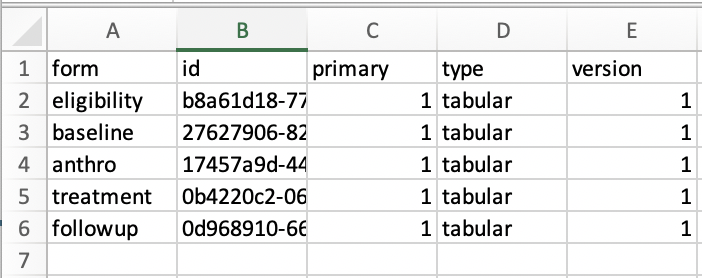
\includegraphics[width=0.6\linewidth,height=0.4\textheight]{images/report-images/api_meta}

\(~\)

\section{Data cleaning/processing}\label{data-cleaningprocessing}

I won't focus explicitly on data cleaning and processing since this process is usually fairly project specific. Briefly, after reading data into R, spend some time making sure all relevant variables (columns) were loaded and checking that variable classes are encoded as expected. Below is an example that checks the structure of the data and converts all variables that should be ``Date'' class to be so.

\begin{verbatim}
#convert all variables with "date" within the name to date class
dt.anthro %<>% mutate_at(vars(matches("date")), as.Date)

#convert all values within "childID" variable to lowercase
dt.anthro %<>% mutate_at(vars(matches("childID")), tolower)
\end{verbatim}

\(~\)

\section{Data monitoring}\label{data-monitoring}

Now that we have data read into R and structured appropriately, we can focus on the (2) primary aims of the report: data validation to be used internally and DSMC-style presentation of the data. Of course the aims of your report may vary but the monitoring examples below represent evaluations critical to almost any RCT.

\subsection{Data validation}\label{data-validation}

\subsubsection{Missing/inappropriately structured data}\label{missinginappropriately-structured-data}

While not the most glamorous component of the report, checking for missing data is critical. It's helpful once all the data have been read in, to conduct some important checks of the data integrity. Did R (or python, etc) correctly interpret and load the data files? Are there any participant IDs missing? Are there participant's with reported birthdates in the future? This is an important stage to think about the plethora of maladies that could befall the data in between when it was recorded and when it got to you. Below are examples of how you could check for some common issues.

\begin{verbatim}
#check for missing values across all columns
map(dt.anthro, ~sum(is.na(.)))

#check for missing values in childsex
na_childSex <- sum(is.na(dt.anthro$childSex))

There are 4 rows with missing values for child sex.
\end{verbatim}

\(~\)

\subsubsection{Reporting inconsistencies}\label{reporting-inconsistencies}

Many studies may use multiple independent questionnaires to gather information at different timepoints and ask the same demographic information. For example, in an individually randomized trial, each participant receives an ID that links the participant responses across all timepoints of the study. Below is an example showing how to check that the responses are consistent across all questionnaires.

\begin{verbatim}
#join anthro and swabs data by childID to check where childSex is different
dt.anthro %>%
  select(childSex, childID) %>%
  inner_join(
    dt.swabs %>% select(childSex, childID),
    by="childID"
  ) %>%
  filter(childSex.x!=childSex.y)
\end{verbatim}

Another component of data validation is checking for overt errors and outliers, many of which can often be fixed in the field. One example is when interviewers may accidentally record a study participant's weight in kilograms instead of grams, resulting in an error 3 magnitudes in size. This error is easily identified (red circle) from plotting the distribution of the birthweights in a histogram.

\begin{verbatim}
#age histogram
dt.anthro %>%
  mutate(weeks = difftime(startTime, date_of_birth, units = "weeks")) %>%
  ggplot(dt.anthro, aes(weeks)) +
    geom_histogram(binwidth = .2) +
    theme_bw() +
    xlab("Age (weeks)") +
    ylab("Count")
\end{verbatim}

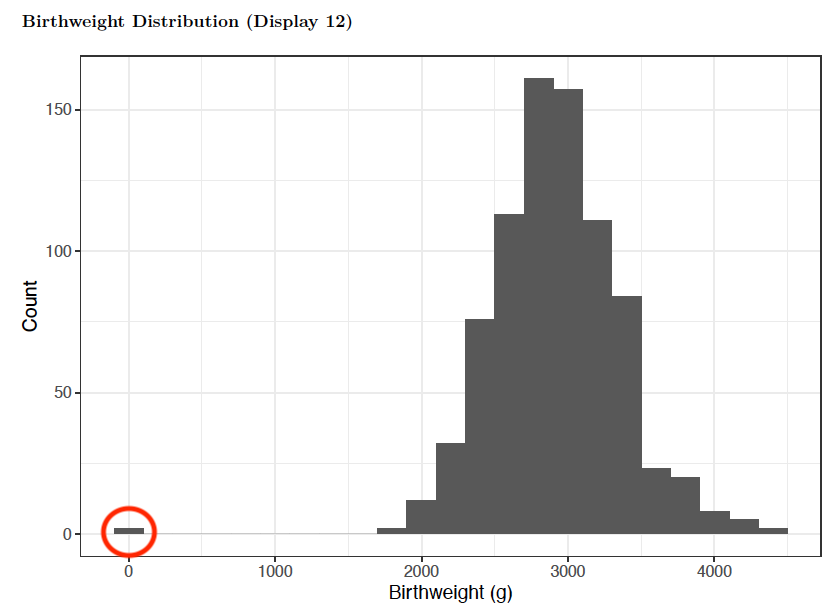
\includegraphics[width=0.6\linewidth,height=0.4\textheight]{images/report-images/birthweight}

Distribution of participant birthweights in grams

\(~\)

\subsection{Data presentation (DSMC-style)}\label{data-presentation-dsmc-style}

The ultimate arbiter of whether a trial remains running is often the Data and Safety Monitoring Committee (DSMC) and these reports can be used to present preliminary findings/analyses as well as detail all relevant safety metrics.

\subsubsection{Enrollment}\label{enrollment}

Any study investigator cares a lot about enrollment, since it determines the length and cost of the trial, among other things. Therefore, any report needs tables/figures showing enrollment trends and trajectory. Below are a couple examples of what they can look like.

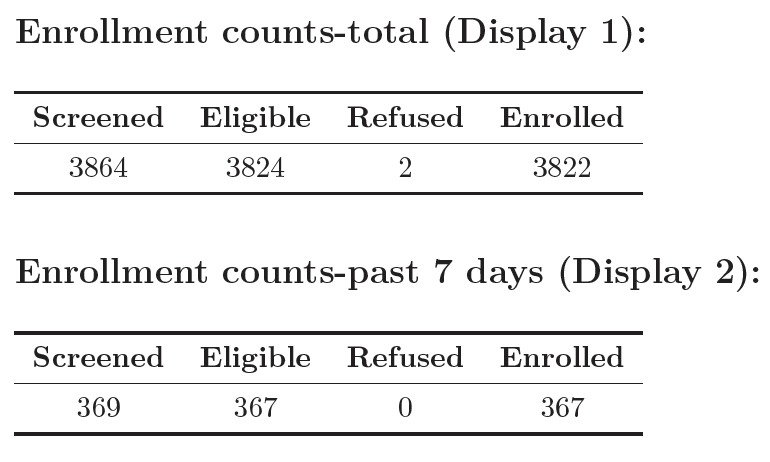
\includegraphics[width=0.5\linewidth,height=0.3\textheight]{images/report-images/enrollment1}

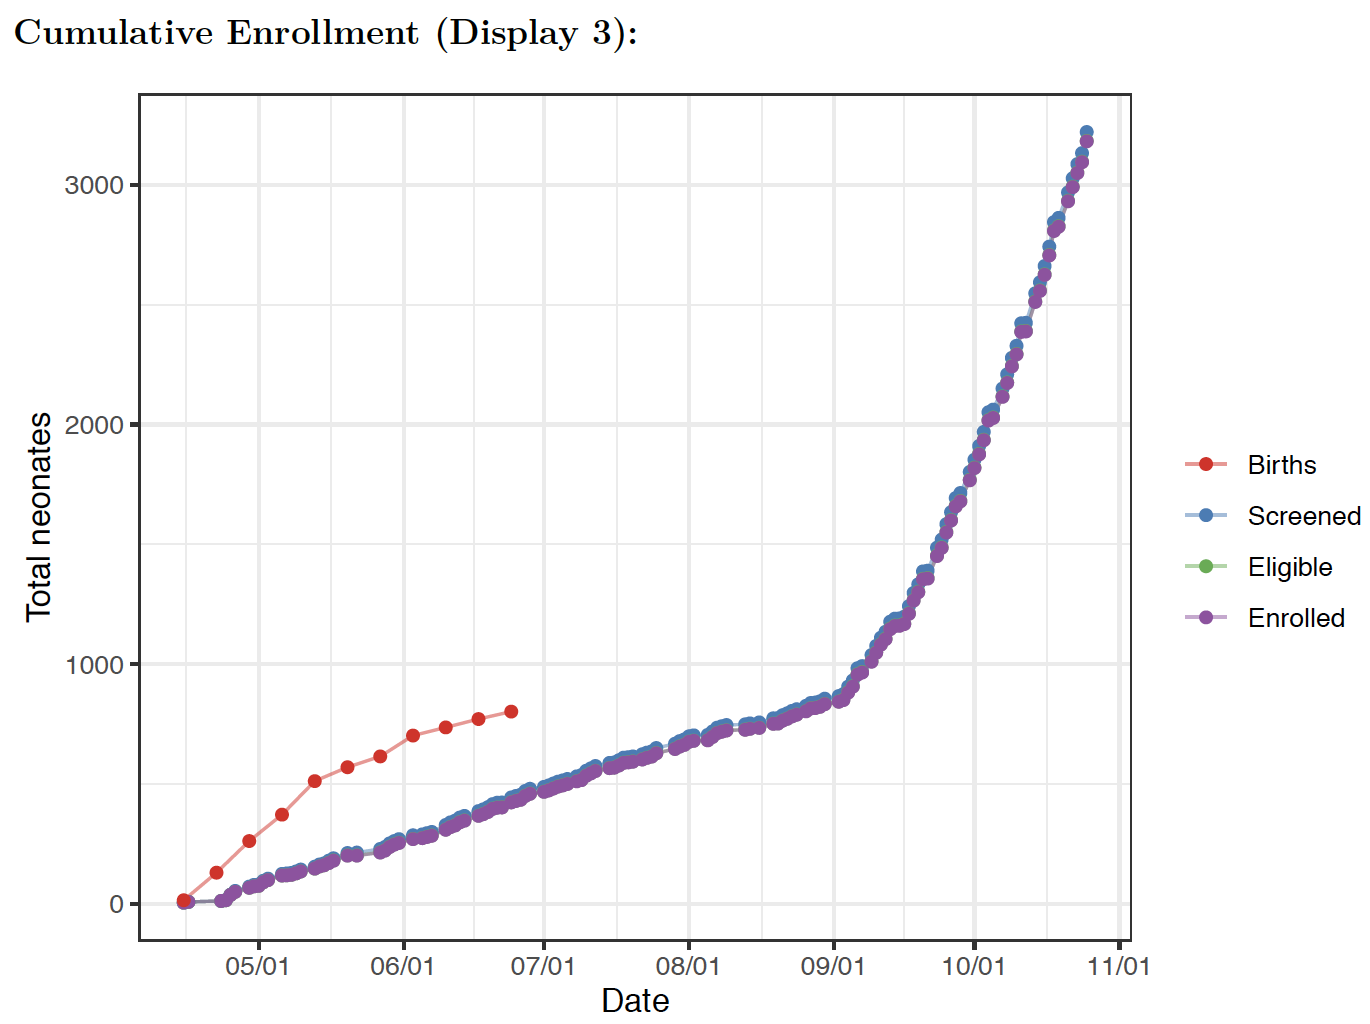
\includegraphics[width=0.7\linewidth,height=0.5\textheight]{images/report-images/enrollment2}

Enrollment counts across the length of the study period.

\(~\)

\subsubsection{Baseline characteristics}\label{baseline-characteristics}

Demographic characteristics of the enrolled participants at baseline are often necessary.

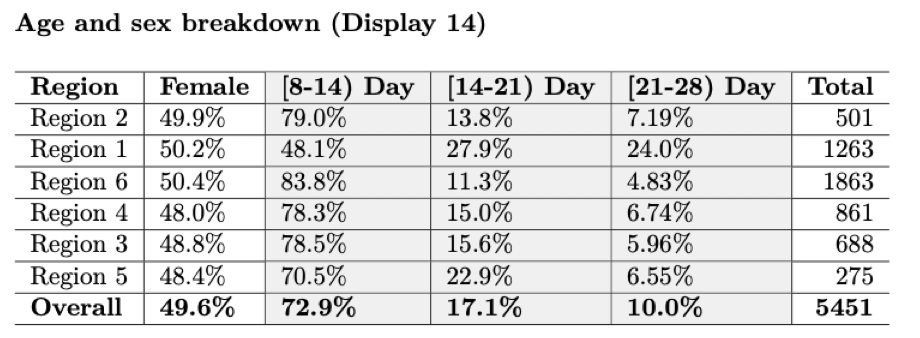
\includegraphics[width=0.6\linewidth,height=0.4\textheight]{images/report-images/baseline}

\(~\)

\subsubsection{Treatment}\label{treatment}

There is usually a treatment component to an RCT, where participants are treated according to their assigned arm (i.e.~treatment or placebo). The report should include checks that confirm particpants actually received the treatment that they were randomized to. Otherwise, the results of the study lack interpretability and are likely null.

\begin{verbatim}
#merge with treatment letters
wrong_random <- dt.treatment %>%
  left_join(dt_letters, by="childID") %>%
  #the treatment letter does not match what's in database
  tally(TL != assignment) %>% as.numeric()

Number of IDs where treatment letter given does not match database: 0
\end{verbatim}

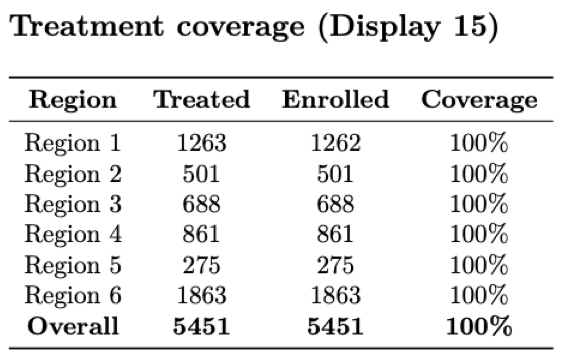
\includegraphics[width=0.4\linewidth,height=0.2\textheight]{images/report-images/treatment}

Counts of number treated and number eligible, along with percent treated (coverage), by region.

\(~\)

\subsubsection{\texorpdfstring{Primary/secondary outcomes (\textbf{\emph{masked!}})}{Primary/secondary outcomes (masked!)}}\label{primarysecondary-outcomes-masked}

This is probably the most exciting section for an investigator to see since these metrics are the motivation of the trial itself. Be especially vigilient to make sure that the figures remain masked when sending to trial investigators and coordinators. This means making sure that you send no information regarding the treatment assignments while the trial is still active.

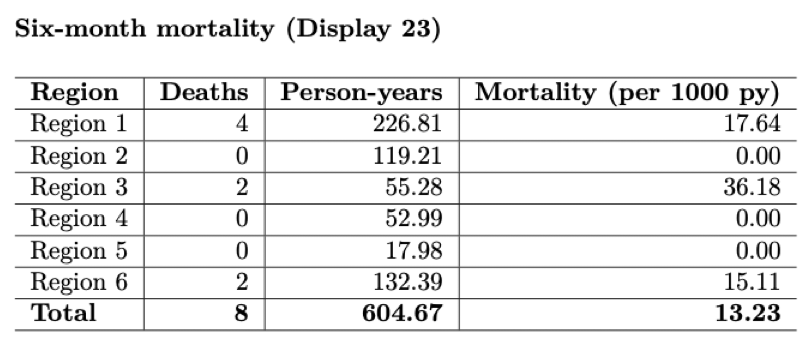
\includegraphics[width=0.5\linewidth,height=0.35\textheight]{images/report-images/primary_outcome}

Preliminary mortality rate and total person-years by region.

\(~\)

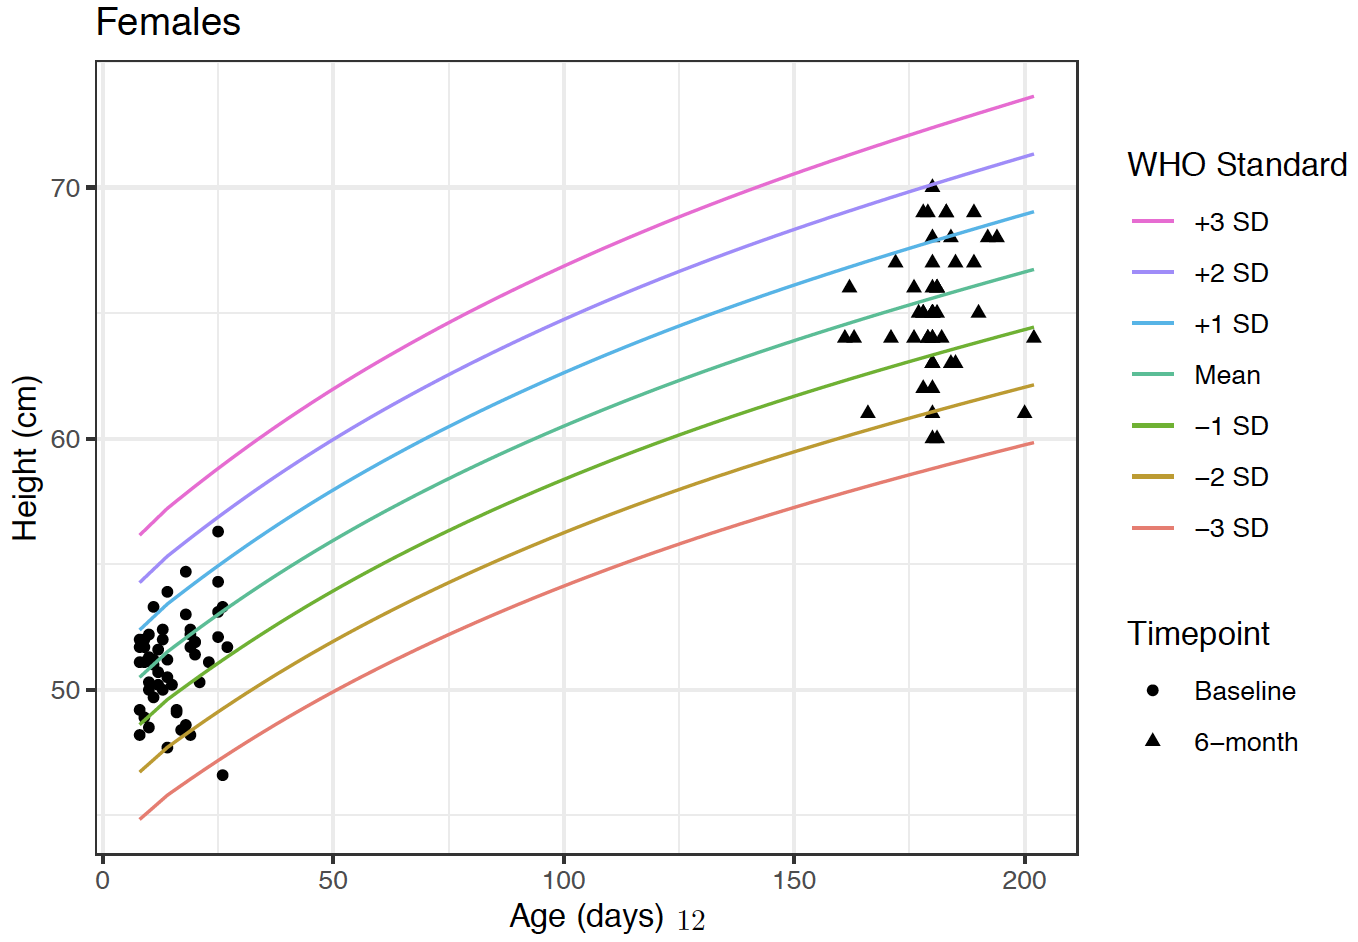
\includegraphics[width=0.5\linewidth,height=0.4\textheight]{images/report-images/growth_curves}

Height growth curves of participants at Baseline and 6-month timepoints.

\(~\)

\subsubsection{Follow-up/Adverse events}\label{follow-upadverse-events}

This report can serve as guard against loss to follow-up, an issue that plagues many trials. By actively monitoring the number of participants that have, and have not, been followed-up on, we can communicate where participants or clusters need to more attention to workers in the field. Below is an example showing follow-up percentages by region.

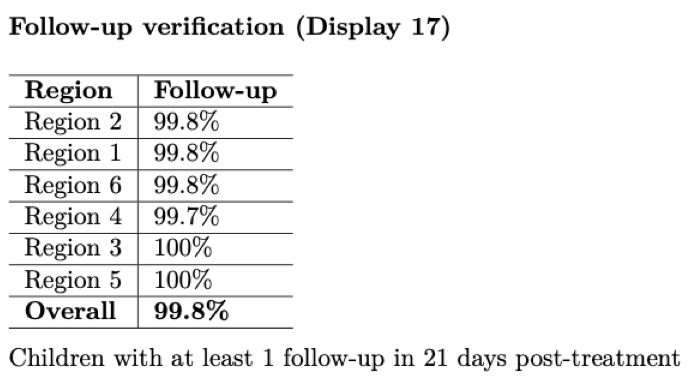
\includegraphics[width=0.5\linewidth,height=0.35\textheight]{images/report-images/followup}

As mentioned above, adverse events should be tabulated and closely watched throughout the study to monitor if the intervention may be causing increased harm.

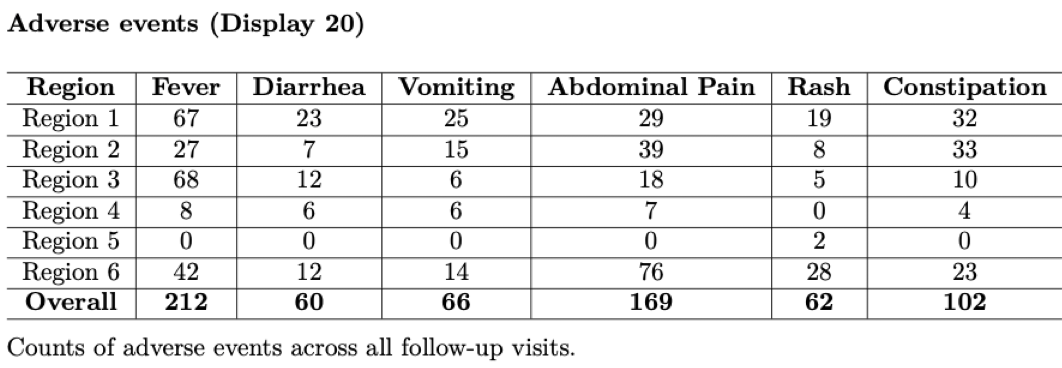
\includegraphics[width=0.65\linewidth,height=0.45\textheight]{images/report-images/adverse_events}

\(~\)

\subsection{Appendix (if necessary)}\label{appendix-if-necessary}

Sometimes an appendix can be helpful to display long lists or addendums to tables shown earlier in the report. Below is an example of a list enumerating all adverse events that were not included in the AE table within the main report.

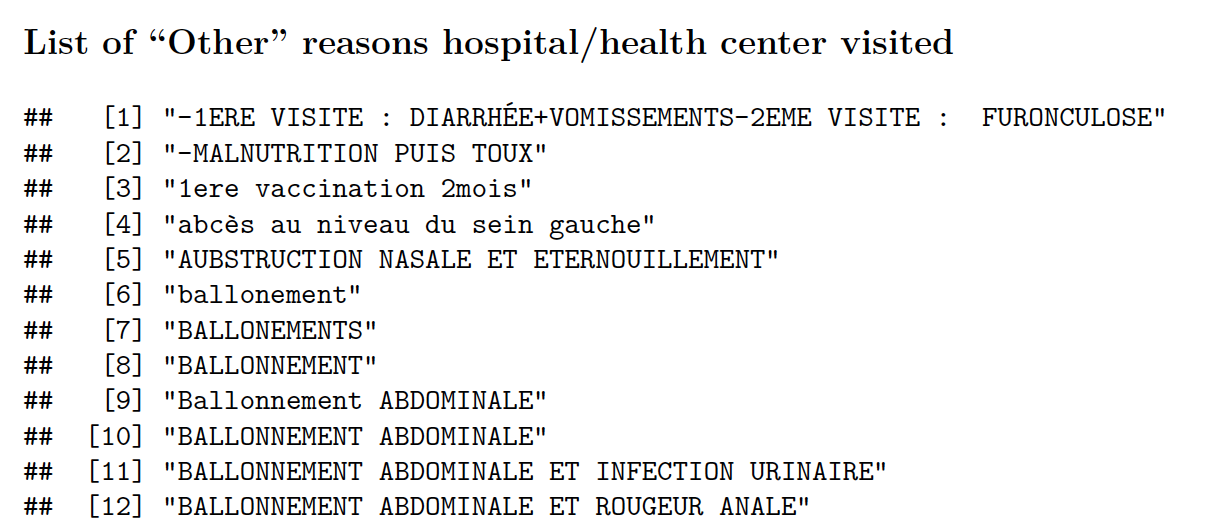
\includegraphics[width=0.7\linewidth,height=0.5\textheight]{images/report-images/appendix}

\(~\)

\section{Summary}\label{summary}

This chapter described and illustrated an example of a data monitoring report using R markdown. This is, by no means, an exhaustive list of what to include in a monitoring report but meant to serve as a template as you create your own report. It is specifically geared towards continuous monitoring of randomized-controlled trials but the overarching concepts apply to other types of trials or even retrospective analyses.

\chapter{Communication and Coordination}\label{commcoord}

\emph{Contributors: Jade Benjamin-Chung, Ben Arnold}

\textbf{These communications guidelines are evolving as we increasingly adopt Slack, but here some general principles if you work closely with Ben.}

\section{Slack}\label{slack}

\begin{itemize}
\item
  If you work with Ben but are not a member of Proctor's Slack workspace then ask him to invite you!
\item
  We do not recommend using Slack for messages you'd like to save and find again in 6 months -- for messages with important information and documentation that you will need in the future, use email!
\item
  Use Slack for scheduling, coding related questions, quick check ins, etc. If your Slack message exceeds 200 words, it might be time to use email.
\item
  Use channels instead of direct messages unless you need to discuss something private.
\item
  Include tags on your message (e.g., \texttt{@Ben}) when you want to ensure that a person sees the message. Ben doesn't regularly read messages where he isn't tagged.
\item
  Please make an effort to respond to messages that message you (e.g., \texttt{@Ben}) as quickly as possible and always within 24 hours, unless of course you are on vacation!
\item
  If you are unusually busy (e.g., taking MCAT/GRE, taking many exams) or on vacation please alert the team in advance so we can expect you not to respond at all / as quickly as usual and also \href{https://get.slack.help/hc/en-us/articles/201864558-Set-your-Slack-status-and-availability}{set your status in Slack} (e.g., it could say ``On vacation'') so we know not to expect to see you online.
\item
  Please thread messages in Slack as much as possible.
\end{itemize}

\section{Email}\label{email}

\begin{itemize}
\tightlist
\item
  Use email for longer messages (\textgreater200 words) or messages that merit preservation.
\item
  Generally, strive to respond within 24 hours. If you are unusually busy or on vacation please alert the team in advance so we can expect you not to respond at all / as quickly as usual.
\end{itemize}

\section{Trello}\label{trello}

\begin{itemize}
\tightlist
\item
  Ben manages projects and teams using a \href{https://www.atlassian.com/agile/kanban/boards}{kanban board approach} in \href{https://www.trello.com}{Trello}.
\item
  You and/or Ben will add new cards within our team's Trello boards and assign them to team members.
\item
  Each card represents a discrete chunk of work.
\item
  Cards higher in a list are higher priority.
\item
  Strive to complete the tasks in your card by the card's due date. Talk to Ben about deadlines -- we can always manage the calendar!
\item
  Use checklists to break down a task into smaller chunks. Usually, you can do this yourself (but ask Ben if you ever want input).
\item
  Move cards to the ``DONE'' list on a board when they are done.
\end{itemize}

\section{Google Drive}\label{google-drive}

\begin{itemize}
\tightlist
\item
  We mostly use Google Drive to create shared documents with longer descriptions of tasks. These documents are linked to Trello cards. Ben often shares these docs with a whole project team since tasks are overlapping, and even if a task is assigned to one person, others may have valuable insights.
\item
  Please invite both of Ben's email addresses to any documents you create (\href{mailto:bfarnold@gmail.com}{\nolinkurl{bfarnold@gmail.com}}, \href{mailto:ben.arnold@ucsf.edu}{\nolinkurl{ben.arnold@ucsf.edu}}).
\end{itemize}

\section{Calendar / Meetings}\label{calendar-meetings}

\begin{itemize}
\tightlist
\item
  Ben will schedule most meetings through the calendar.
\item
  Our meetings start on the hour.
\item
  If you are going to be late, please send a message in our Slack channel.
\item
  If you are regularly not able to come on the hour, notify the team and we might choose the modify the agenda order or the start time.
\item
  Add hoc meetings are welcome. If Ben's office door is open, come in!
\end{itemize}

\chapter{Code of conduct}\label{code-of-conduct}

\emph{Contributors: Jade Benjamin-Chung, Ben Arnold}

\section{Group culture}\label{group-culture}

We strive to work in an environment that is collaborative, supportive, open, and free from discrimination and harassment, per University policies.

We encourage students / staff of all experience levels to respectfully share their honest opinions and ideas on any topic. Our group has thrived upon such respectful honest input from team members over the years, and this document is a product of years of student and staff input (and even debate) that has gradually improved our productivity and overall quality of our work.

If Ben is your PI, be forewarned that he tends to batch his email communication (\textasciitilde30 mins in the morning and afternoon, 15 mins mid-day), and doesn't tend to answer Slack or email during evenings or weekends. If you need to reach him urgently then give him a call or text on his mobile.

\section{Protecting human subjects}\label{protecting-human-subjects}

All lab members must complete \href{https://irb.ucsf.edu/citi-human-subjects-training}{CITI Human Subjects Training} and share their certificate with Ben. We will will add team members to relevant Institutional Review Board protocols to ensure they have permission to work with identifiable datasets.

One of the most relevant aspects of protecting human subjects in our work in the Data Coordinating Center is maintaining confidentiality and data privacy. For students supporting our data science efforts, in practice this means:

\begin{itemize}
\tightlist
\item
  If you are using a virtual computer (e.g., Google Cloud, AWS, Optum), never save the data in that system to your personal computer or any other computer without prior permission.
\item
  Do not share data with anyone without first obtaining permission, including to other members of the Proctor Foundation, who might not be on the same IRB protocol as you (check with Ben or the relevant PI first).
\item
  \textbf{NEVER} push a dataset into the public domain (e.g., GitHub, OSF) without first checking with Ben to ensure that it is appropriately de-identified and we have approval from the sponsor and/or human subjects review board to do so.
\end{itemize}

Remember, data that looks like it does not contain identifiers to you might still be classified as data that requires special protection by our IRB or under HIPAA, so always proceed with caution and ask for help if you have any concerns about how to maintain study participant confidentiality. For example, the combination of age, sex, and geographic location of the individual's town or neighborhood is typically considered identifiable.

\section{Authorship}\label{authorship}

We adhere to the \href{http://www.icmje.org/recommendations/browse/roles-and-responsibilities/defining-the-role-of-authors-and-contributors.html}{ICMJE Definition of authorship} and are happy for team members who meet the definition of authorship to be included as co-authors on scientific manuscripts.

\section{Work hours}\label{work-hours}

Please follow the Proctor Foundation's employee guidelines for work hours, and discuss the specifics with your PI. If Ben is your PI, then work with him on your schedule to ensure we have overlap in the office and that you are around at key times for group meetings, etc.

\chapter{Additional Resources}\label{resources}

TBD

  \bibliography{book.bib,packages.bib}

\end{document}
